%%%%%%%%%%%%%%%%%%%%%%%% PACKAGES %%%%%%%%%%%%%%%%%%%%%%%%%%%%%%%
%%%%%%%%%%%%%%%%%%%%%%%%%%%%%%%%%%%%%%%%%%%%%%%%%%%%%%%%%%%%%%%%%
% {
\documentclass[a4paper]{report}
\usepackage{minted}
\setminted{
    breaklines=true,
    fontsize=\small
}
\usepackage{xurl}
\usepackage{a4wide,amssymb,epsfig,latexsym,multicol,array,hhline,fancyhdr}
\usepackage{vntex}
%\usepackage[utf8]{vietnam}
\usepackage{amsmath}
\usepackage{lastpage}
\usepackage[lined,boxed,commentsnumbered]{algorithm2e}
\usepackage{enumerate}
\usepackage{xcolor}
\usepackage{graphicx}  % Standard graphics package
\usepackage{array}
\usepackage{tabularx, caption}
\usepackage{multirow}
\usepackage{multicol}
\usepackage{rotating}
\usepackage{graphics}
\usepackage{geometry}
\usepackage{setspace}
\usepackage{epsfig}
\usepackage{tikz}
\usepackage{cite}
\usetikzlibrary{shapes.geometric, arrows}

\tikzstyle{startstop} = [rectangle, rounded corners, minimum width=3cm, minimum height=1cm,text centered, draw=black, fill=black!10]
\tikzstyle{process} = [rectangle, minimum width=3cm, minimum height=1cm, text centered, draw=black, fill=blue!10]
\tikzstyle{decision} = [diamond, minimum width=3cm, minimum height=1cm, text centered, draw=black, fill=green!10]
\tikzstyle{data} = [trapezium, trapezium left angle=70, trapezium right angle=110, minimum width=3cm, minimum height=1cm, text centered, draw=black, fill=red!10]
\tikzstyle{arrow} = [thick,->,>=stealth]

\definecolor{framecolor}{RGB}{58, 108, 189}  %Định nghĩa màu xanh dương
\usetikzlibrary{calc}   %thư viện tikz
\usepackage{xfrac}
\usepackage{bm}
\usepackage{indentfirst}
\usepackage{float}%move tables/ images
\usepackage{titlesec} 
%\usepackage{caption}
\renewcommand{\baselinestretch}{1}
\setlength{\parskip}{0.25cm} %khoảng cách các đoạn
% \usepackage{biblatex}
\usepackage[colorlinks]{hyperref}
% \usepackage[acronym,toc]{glossaries}
% \usepackage[symbols,nogroupskip,nonumberlist]{glossaries-extra}
\usepackage[
 sort=none,% no sorting or indexing required
 abbreviations,% create list of abbreviations
 symbols,% create list of symbols
 stylemods,style=list, % set the default glossary style
 nogroupskip, nonumberlist, nomain
]{glossaries-extra}
\usepackage{booktabs}
\usepackage{subcaption}
\usepackage{amsmath}
\usepackage{url}
%%%%%%%%%%%%%%%%%%%%%%%%%%%%%%%%%%%%%%%%%%%%%%%%%%%%%%%%%%%%%%%%%%
%%%%%%%%%%%%%%%%%%%%%%%% FORMATTING %%%%%%%%%%%%%%%%%%%%%%%%%%%%%
%%%%%%%%%%%%%%%%%%%%%%%%%%%%%%%%%%%%%%%%%%%%%%%%%%%%%%%%%%%%%%%%%%
% {
\DeclareMathOperator{\arccot}{arccot}
\captionsetup[table]{name=Table}
\captionsetup[figure]{name=Figure}
\newenvironment{Description}{\list{}{%
    \let\makelabel\descriptionlabel    % this comes from the original description environment
    \setlength{\rightmargin}{\leftmargin}% this comes from the original quote environment
    \setlength{\labelwidth}{0pt}%          this is new
    }}{\endlist}

\usemintedstyle{default} 

    
\hypersetup{urlcolor=blue,linkcolor=black,citecolor=black,colorlinks=true} 
\usetikzlibrary{arrows,snakes,backgrounds}
\usetikzlibrary{shapes, arrows, positioning}
\definecolor{mathblue}{RGB}{0,114,188}
% \makeatletter  \def\m@th{\mathsurround\z@\color{mathblue}} \makeatother
% \everymath{\color{mathblue}}
% \setmathfont[Color=000000]{Arial}
%\usepackage{pstcol} 								% PSTricks with the standard color package
\newtheorem{theorem}{{\bf Theorem}}
\newtheorem{property}{{\bf Property}}
\newtheorem{proposition}{{\bf Proposition}}
\newtheorem{corollary}[proposition]{{\bf Corollary}}
\newtheorem{lemma}[proposition]{{\bf Lemma}}

\AtBeginDocument{\renewcommand{\listfigurename}{Danh sách hình ảnh}}
\AtBeginDocument{\renewcommand{\listtablename}{Danh sách bảng}}
\AtBeginDocument{\renewcommand*\contentsname{Mục lục}}
\AtBeginDocument{\renewcommand*\refname{Tài liệu tham khảo}}
%\usepackage{fancyhdr}

%%%%%%%%%%%%%%%%%% SET HEADER AND FOOTER %%%%%%%%%%%%%%%%%%%%%%%%

\setlength{\headheight}{40pt}
\pagestyle{fancy}
\fancyhead{} % clear all header fields
\fancyhead[L]{
 \begin{tabular}{rl}
    \begin{picture}(25,15)(0,0)
    \put(0,-8){\includegraphics[width=8mm, height=8mm]{hcmut.png}}
    %\put(0,-8){\epsfig{width=10mm,figure=hcmut.eps}}
   \end{picture}&
	%\includegraphics[width=8mm, height=8mm]{hcmut.png} & %
	\begin{tabular}{l}
		\textbf{\bf \ttfamily Trường Đại học Bách Khoa - ĐHQG-HCM}\\
		\textbf{\bf \ttfamily Khoa Khoa học và Kỹ thuật máy tính}
	\end{tabular} 	
 \end{tabular}
}
\fancyhead[R]{
	\begin{tabular}{l}
		\tiny \bf \\
		\tiny \bf 
	\end{tabular}  }
\fancyfoot{} % clear all footer fields
\fancyfoot[L]{\scriptsize\ttfamily Báo cáo Đồ án tổng hợp - Học kỳ 251 - Năm học 2025 - 2026}
\fancyfoot[R]{\scriptsize \ttfamily Trang {\thepage}/\pageref{LastPage}}
\renewcommand{\headrulewidth}{0.3pt}
\renewcommand{\footrulewidth}{0.3pt}

\setcounter{secnumdepth}{4}
\setcounter{tocdepth}{4}

\makeatletter
\newcounter {subsubsubsection}[subsubsection]
\renewcommand\thesubsubsubsection{\thesubsubsection .\@arabic\c@subsubsubsection}
\newcommand\subsubsubsection{\@startsection{subsubsubsection}{4}{\z@}%
                                     {-3.25ex\@plus -1ex \@minus -.2ex}%
                                     {1.5ex \@plus .2ex}%
                                     {\normalfont\normalsize\bfseries}}
\newcommand*\l@subsubsubsection{\@dottedtocline{3}{10.0em}{4.1em}}
\newcommand*{\subsubsubsectionmark}[1]{}
% \def\m@th{\mathsurround\z@\color{mathblue}}
\makeatother
% }
% }
%%%%%%%%%%%%%%%%%%%%%%%%%%%%%%%%%%%%%%%%%%%%%%%%%%%%%%%%%%%%%%%%%%
% ACRONYMS & SYMBOLS
% {
% \makeglossaries
\setabbreviationstyle{long-short}
\newabbreviation{fig}{Fig.}{Figure}
\newabbreviation{tab}{Tab.}{Table}
\newabbreviation{eq}{Eq.}{Equation}
\newabbreviation{eg}{e.g.}{For Example}
\newabbreviation{ie}{i.e.}{That Is}
% \glsnoexpandfields
%\glsxtrnewsymbol[description = {: Tập hợp số tự nhiên}]{natural}{\ensuremath{\mathbb{N}}}
% }
%%%%%%%%%%%%%%%% Thiết lập định dạng cho section %%%%%%%%%%%%%%%%%
\titleformat{\section}
 {\fontsize{13}{15}\bfseries} % Kích thước font là 13pt, in đậm
 {\thesection.} % Số thứ tự section với dấu chấm
 {5pt} % Khoảng cách giữa số thứ tự và tiêu đề
 {} % Format trước tiêu đề
\titleformat{\subsection}
 {\fontsize{13}{13}\bfseries}
 {\hspace{1em}\thesubsection.}
 {5pt}
 {}
\titleformat{\subsubsection}
 {\fontsize{13}{13}\bfseries}
 {\hspace{1.5em}\thesubsubsection.}
 {5pt}
 {}
 \titleformat{\subsubsubsection}
 {\fontsize{13}{13}\bfseries}
 {\hspace{1.5em}\thesubsubsubsection/}
 {5pt}
 {}
\titlespacing*{\section} % Áp dụng cho \section
{0pt}  % Lề trái (left margin)
{0pt} % Khoảng cách trước tiêu đề (before the title)
{0pt} % Khoảng cách sau tiêu đề (after the title)
%%%%%%%%%%%%%%%%%%%%%%%%%%%%%%%%%%%%%%%%%%%%%%%%%%%%%%%%%%%%%%%%%
%%%%%%%%%%%%%%%%%%%%%%%%%% DOCUMENT %%%%%%%%%%%%%%%%%%%%%%%%%%%%%
%%%%%%%%%%%%%%%%%%%%%%%%%%%%%%%%%%%%%%%%%%%%%%%%%%%%%%%%%%%%%%%%%
% Math operators
\newcommand{\project}{\pi}
\newcommand{\select}{\sigma}
\newcommand{\join}{\bowtie}
\newcommand{\rename}{\rho}
\newcommand{\group}{\mathcal{F}}
\newcommand{\sub}{\textsubscript}

\begin{document}

% --- Bắt đầu đánh số La Mã cho phần đầu (i, ii, iii...) ---
\pagenumbering{roman}
%%%%%%%%%%%%%%%%%%%%%%%%% TITLE PAGE %%%%%%%%%%%%%%%%%%%%%%%%%%%%
\begin{titlepage}

\begin{tikzpicture}[overlay, remember picture]
\draw [line width = 3pt, framecolor]
    ($ (current page.north west) + (2.0cm, -2.0cm) $)
    rectangle
    ($ (current page.south east) + (-2.0cm, 2.0cm) $);
\draw [line width = 1pt, framecolor]
    ($ (current page.north west) + (2.15cm, -2.15cm) $)
    rectangle
    ($ (current page.south east) + (-2.15cm, 2.15cm) $);
\end{tikzpicture}

\vspace{-0.7cm}

\begin{center}
\Large
\textbf{ĐẠI HỌC QUỐC GIA THÀNH PHỐ HỒ CHÍ MINH} \\
\textbf{TRƯỜNG ĐẠI HỌC BÁCH KHOA} \\
\textbf{KHOA KHOA HỌC VÀ KỸ THUẬT MÁY TÍNH}
\end{center}

\vspace{0.7cm}

\begin{figure}[h!]
\begin{center}
\includegraphics[width=5cm]{hcmut.png}
\end{center}
\end{figure}

\vspace{0.4cm}


\begin{center}
\begin{tabular}{c}
\multicolumn{1}{c}{\textbf{{\Large BÁO CÁO ĐỒ ÁN TỔNG HỢP}}}\\
\\
\hline
% \multicolumn{1}{l}{\textbf{{\Large Bài tập lớn}}}\\
\\



\parbox{0.9\textwidth}{\centering \textbf{\textit{{\huge “Nghiên cứu và so sánh phương pháp Weak Supervision và Supervised Learning trong phân tích cảm xúc lĩnh vực Gaming”}}}}\\
\\
\hline
\end{tabular}
\end{center}

\vspace{0.2cm}
\begin{table}[h]
\Large
\centering
    \begin{tabular}{rl}
    \hspace{1.7 cm}\textbf{GVHD}:
    & Tiến sĩ Nguyễn An Khương \\
    %& ThS. Mai Xuân Toàn\\
    & \\
    \textbf{Sinh viên}: &Nguyễn Thành Công - 2310373 \\
    &  Lê Thúy Hiền - 2310990 \\
    \end{tabular}
\end{table}
\vspace{0.2cm}
\begin{center}
{\normalsize  THÀNH PHỐ HỒ CHÍ MINH, THÁNG 11 - 2025}
\end{center}
\end{titlepage}
%%%%%%%%%%%%%%%%%%%%%%%%%%%%%%%%%%%%%%%%%%%%%%%%%%%%%%%%%%%%%%%%%
\pagebreak

\tableofcontents
\pagebreak

\pagebreak
\listoffigures
\listoftables

\addcontentsline{toc}{section}{Danh sách hình ảnh}
\addcontentsline{toc}{section}{Danh sách bảng}

\renewcommand{\arraystretch}{1.5} % Tăng hệ số khoảng cách dòng (1.5 là ví dụ)
\pagebreak



\section*{Danh sách thành viên \& nhiệm vụ}
\addcontentsline{toc}{section}{Danh sách thành viên \& nhiệm vụ}
\begin{center}
\begin{table}[h]
\centering
\begin{tabular}{|c|c|c|p{5cm}|c|}
\hline
\textbf{STT} & \textbf{Họ và tên} & \textbf{MSSV} & \textbf{ Nhiệm vụ} & \textbf{\% hoàn thiện}\\
\hline 
%%%%% Student 1 (Hằng) %%%%%%%%%%
\multirow{3}{*}{1} & \multirow{3}{*}{Lê Thúy Hiền} & \multirow{3}{*}{2310990} & 
- Code stage 2 \& stage 3b & \multirow{3}{*}{100\%}\\
 & &  & - Báo cáo chương 3, 4, 5, 6 &\\
 & &  & - Slide thuyết trình &\\
\hline
\multirow{3}{*}{2} & \multirow{3}{*}{Nguyễn Thành Công} & \multirow{3}{*}{2310373} & 
- Code stage 1 \& stage 3a & \multirow{3}{*}{100\%}\\
& &  & - Báo cáo chương 1, 2, 3 &\\
 & &  & - Slide thuyết trình &\\

\hline
\end{tabular}
\caption{\label{Bảng 1}Danh sách thành viên \& nhiệm vụ}
\end{table}
\end{center}
\pagebreak


\clearpage % Ngắt trang để đảm bảo chương 1 bắt đầu trang mới
\pagenumbering{arabic} % Chuyển sang số 1, 2, 3...
\setcounter{page}{1}   % Đặt lại bộ đếm về 1

% ============================================================================
% CHƯƠNG 1: TỔNG QUAN (INTRODUCTION)
% ============================================================================

\chapter{TỔNG QUAN}

\section{Đặt vấn đề}

Trong kỷ nguyên số hóa hiện nay, ngành công nghiệp trò chơi điện tử (gaming) đang chứng kiến sự phát triển bùng nổ với quy mô thị trường toàn cầu đạt hàng trăm tỷ USD. Cùng với sự phát triển này là lượng nội dung đánh giá, thảo luận về game trên các nền tảng mạng xã hội tăng theo cấp số nhân. Các nền tảng như \textbf{Reddit} (với các subreddit gaming lớn như r/gaming, r/Games, r/pcgaming), \textbf{Steam}, \textbf{Metacritic}, và \textbf{Twitter} mỗi ngày tiếp nhận hàng triệu bài viết, bình luận từ cộng đồng người chơi.

Việc phân tích cảm xúc (sentiment analysis) từ khối lượng dữ liệu khổng lồ này mang lại giá trị to lớn cho nhiều đối tượng: các nhà phát triển game có thể nắm bắt phản hồi cộng đồng để cải thiện sản phẩm, nhà phân phối có thể đánh giá xu hướng thị trường, và người tiêu dùng có thể tham khảo đánh giá trước khi mua game. Tuy nhiên, việc áp dụng các phương pháp sentiment analysis truyền thống vào lĩnh vực gaming gặp phải ba thách thức đặc thù:

\subsection{Thách thức 1: Đặc trưng ngôn ngữ gaming phức tạp}

Ngôn ngữ được sử dụng trong cộng đồng game thủ mang những đặc điểm chuyên biệt, khác xa với ngôn ngữ phổ thông, tạo ra rào cản lớn cho các phương pháp phân tích cảm xúc truyền thống. Đầu tiên là sự xuất hiện dày đặc của các thuật ngữ kỹ thuật (technical jargon) như \textbf{"FPS drop"}, \textbf{"input lag"} hay \textbf{"hitbox"}; đòi hỏi mô hình phải hiểu được ngữ nghĩa chuyên ngành thay vì nghĩa đen thông thường. Bên cạnh đó, hệ thống tiếng lóng (slang) và từ viết tắt như \textbf{"P2W"} (pay-to-win) hay \textbf{"GOTY"} (Game of the Year) phát triển mạnh mẽ và thay đổi liên tục theo xu hướng. Khó khăn hơn cả là tính đa nghĩa theo ngữ cảnh (contextual polysemy) và sự phổ biến của lối nói châm biếm (sarcasm). Một từ ngữ mang sắc thái tích cực như \textbf{"masterpiece"} hoặc \textbf{"optimized"} hoàn toàn có thể được sử dụng để biểu đạt sự mỉa mai tiêu cực khi đi kèm với các bối cảnh lỗi game, khiến việc xác định đúng cảm xúc trở nên vô cùng phức tạp.

\subsection{Thách thức 2: Chi phí gán nhãn thủ công cao}

Việc xây dựng bộ dữ liệu huấn luyện chất lượng cao cho mô hình học có giám sát (Supervised Learning) đối mặt với bài toán nan giải về chi phí và khả năng mở rộng. Quá trình gán nhãn thủ công không chỉ đòi hỏi nguồn lực tài chính lớn để thuê chuyên gia có kiến thức nền tảng về game, mà còn tiêu tốn lượng thời gian đáng kể để xử lý hàng chục nghìn bài viết. Hơn nữa, tính nhất quán của dữ liệu thường không được đảm bảo do sự khác biệt trong quan điểm chủ quan của từng người gán nhãn (annotator), đặc biệt đối với các nội dung mang tính subjective. Đặc biệt, với tốc độ sinh dữ liệu khổng lồ hàng ngày trên các nền tảng mạng xã hội, phương pháp thủ công trở nên bất khả thi trong việc đáp ứng nhu cầu cập nhật dữ liệu liên tục ở quy mô lớn.

\subsection{Thách thức 3: Mất cân bằng dữ liệu tự nhiên}

Dữ liệu thực tế trong lĩnh vực gaming thường tồn tại sự mất cân bằng phân phối nghiêm trọng (class imbalance). Do tâm lý hành vi người dùng thường có xu hướng chia sẻ nhiều hơn khi hài lòng, dữ liệu gaming thường gặp hiện tượng "positive bias" với nhãn \textbf{Positive} chiếm đa số (thường dao động 40-50\%), trong khi các đánh giá \textbf{Negative} (Tiêu cực)—nguồn thông tin quan trọng nhất cho nhà phát triển—lại chỉ chiếm tỷ lệ thiểu số (15-20\%). Ngoài ra, lớp \textbf{Neutral} mang tính chất thảo luận hoặc hỏi đáp thường xuyên bị chồng lấn (overlapping) ranh giới với hai lớp còn lại. Sự mất cân bằng này khiến các mô hình học máy truyền thống dễ bị thiên kiến (bias) về phía lớp đa số để tối ưu hóa hàm mất mát, dẫn đến việc bỏ qua hoặc nhận diện kém các đặc trưng quan trọng của lớp thiểu số \cite{lin2017focal}.

% ----------------------------------------------------------------------------
\section{Mục tiêu nghiên cứu}

Nghiên cứu này đặt ra ba mục tiêu chính nhằm giải quyết các thách thức đã nêu:

\subsection{Mục tiêu 1: Xây dựng hệ thống Weak Supervision cho Gaming Domain}

Mục tiêu đầu tiên là phát triển một hệ thống tự động gán nhãn cảm xúc cho nội dung gaming trên Reddit, tận dụng các tín hiệu cộng đồng (community signals) để thay thế quy trình gán nhãn thủ công tốn kém. Quá trình này bao gồm ba bước chính:

Đầu tiên, \textbf{thu thập dữ liệu} được thực hiện bằng cách crawl bài viết từ 6 subreddit gaming lớn bao gồm: r/gaming, r/Games, r/pcgaming, r/gamernews, r/gamedev, và r/indiegaming.

Tiếp theo, đề tài \textbf{thiết kế chiến lược 8-Signal}, kết hợp 8 loại tín hiệu với trọng số khác nhau để suy luận nhãn:
\textbf{Awards} (trọng số 4.0 - tín hiệu mạnh nhất),
\textbf{Comments Count} (3.0 - mức độ engagement),
\textbf{Upvote Ratio} (2.5 - sự đồng thuận),
\textbf{Post Score} (2.0 - độ phổ biến),
\textbf{Gaming Text Features} (1.8-3.0 - từ vựng đặc thù),
\textbf{Sarcasm Detection} (cơ chế đảo chiều sentiment),
\textbf{Flair Analysis} (2.0-3.5 - phân loại từ nhãn bài viết), và
\textbf{Top Comments} (2.0-2.5 - phân tích phản hồi cộng đồng).

Cuối cùng, hệ thống sử dụng \textbf{Weighted Voting Mechanism} để tổng hợp các tín hiệu trên với trọng số động (dynamic weighting từ 1.8 đến 3.5) kèm theo điểm tin cậy (confidence scoring) nhằm tạo ra các nhãn yếu (weak labels) chất lượng cao. Hiệu quả của phương pháp sẽ được đánh giá thông qua việc so sánh Accuracy, F1-score và thời gian huấn luyện với phương pháp Supervised Learning truyền thống.

\subsection{Mục tiêu 2: Giải quyết bài toán Class Imbalance}

Để khắc phục hiện tượng mất cân bằng dữ liệu nghiêm trọng trong lĩnh vực gaming, đề tài nghiên cứu và so sánh hai nhóm phương pháp chính:

\subsubsection{Phương pháp Algorithm-Level (Focal Loss và Class Weighting)}

Đối với hướng tiếp cận ở mức thuật toán, đề tài tập trung vào Focal Loss, một kỹ thuật giúp mô hình tập trung vào các mẫu khó phân loại. Công thức toán học được định nghĩa như sau:

\begin{equation}
    FL(p_t) = -\alpha_t (1 - p_t)^{\gamma} \log(p_t)
\end{equation}

Trong đó, $p_t$ là xác suất dự đoán đúng của mẫu. Tham số $\alpha$ đóng vai trò trọng số cân bằng lớp, trong khi $\gamma$ là tham số tập trung (focusing parameter) giúp giảm trọng số của các mẫu dễ (easy examples) thông qua hệ số điều chỉnh $(1-p_t)^{\gamma}$.

Bên cạnh đó, phương pháp Class Weighting cũng được áp dụng để tích hợp trọng số vào hàm CrossEntropyLoss, trong đó lớp thiểu số sẽ nhận trọng số cao hơn dựa trên công thức:
\begin{equation}
    w_j = \frac{N}{K \cdot n_j}
\end{equation}
Với $N$ là tổng số mẫu, $K=3$ là số lượng lớp, và $n_j$ là số mẫu của lớp $j$. Ưu điểm của phương pháp này là đơn giản hơn Focal Loss do không cần tinh chỉnh các siêu tham số $\alpha, \gamma$.

\subsubsection{Phương pháp Data-Level (Undersampling)}

Ở mức dữ liệu, phương pháp \textbf{Undersampling} được sử dụng làm cơ sở so sánh (baseline). Kỹ thuật này giảm số lượng mẫu của lớp đa số xuống mức cân bằng với lớp thiểu số (từ 21,821 xuống 12,093 mẫu). Mặc dù đảm bảo sự cân bằng hoàn toàn, phương pháp này phải đánh đổi bằng việc mất đi một lượng lớn dữ liệu huấn luyện ($\sim$9,728 mẫu).

\subsection{Mục tiêu 3: So sánh định lượng các phương pháp}

Mục tiêu cuối cùng là xây dựng một pipeline gồm 4 giai đoạn (Stages) để thực hiện so sánh toàn diện giữa Weak Supervision và các chiến lược Supervised Learning:

\begin{figure}[H]
    \centering
    \begin{tikzpicture}[node distance=1cm]
        \node (stage1) [rectangle, draw, text width=3cm, align=center] {Stage 1\\Weak Supervision\\Reddit Gaming};
        \node (stage2) [rectangle, draw, text width=3cm, align=center, right of=stage1, xshift=3cm] {Stage 2\\Balanced\\Undersampling};
        \node (stage3) [rectangle, draw, text width=3cm, align=center, right of=stage2, xshift=3cm] {Stage 3\\Focal Loss/Weighting\\Full Imbalanced};
        \node (stage4) [rectangle, draw, text width=3cm, align=center, right of=stage3, xshift=3cm] {Stage 4\\Comparison\\Analysis};
        
        \draw [->] (stage1) -- (stage2);
        \draw [->] (stage2) -- (stage3);
        \draw [->] (stage3) -- (stage4);
    \end{tikzpicture}
    \caption{Pipeline 4 stages so sánh Weak Supervision và Supervised Learning}
\end{figure}

Các phương pháp sẽ được đánh giá đa chiều dựa trên 5 tiêu chí: (1) \textbf{Accuracy \& F1-Score} (hiệu suất phân loại), (2) \textbf{Training Time} (tốc độ huấn luyện), (3) \textbf{Dataset Efficiency} (mức độ tận dụng dữ liệu), (4) \textbf{Labeling Cost} (chi phí gán nhãn), và (5) \textbf{Per-Class Performance} (hiệu quả trên từng lớp cụ thể: Negative, Neutral, Positive).


% ----------------------------------------------------------------------------
\section{Đối tượng và phạm vi nghiên cứu}

\subsection{Nguồn dữ liệu nghiên cứu}

\subsubsection{Dữ liệu Weak Supervision (Stage 1)}

Để xây dựng bộ dữ liệu huấn luyện cho mô hình Weak Supervision, nghiên cứu tập trung thu thập dữ liệu từ \textbf{Reddit} - nền tảng thảo luận lớn nhất thế giới về gaming. Cụ thể, dữ liệu được crawl từ 6 subreddit tiêu biểu bao gồm: \textbf{r/gaming} ($\sim$35M thành viên), \textbf{r/Games} ($\sim$3M thành viên - tập trung vào thảo luận chất lượng cao), \textbf{r/pcgaming} ($\sim$2.5M thành viên), \textbf{r/gamernews}, \textbf{r/gamedev}, và \textbf{r/indiegaming}.

Các subreddit này được lựa chọn dựa trên các tiêu chí khắt khe nhằm đảm bảo chất lượng dữ liệu: số lượng thành viên đông đảo ($>$100K), tần suất đăng bài cao ($>$100 bài/ngày), tỷ lệ spam thấp ($<$5\%) và mức độ tương tác tốt (tỷ lệ upvote trung bình $>$0.7). Nội dung thảo luận bao phủ đa dạng các chủ đề từ tin tức, review, phát triển game đến trải nghiệm người chơi.

Quá trình thu thập được thực hiện thông qua thư viện \textbf{PRAW} (Python Reddit API Wrapper), giới hạn trong các bài đăng thuộc tháng 11/2025. Các từ khóa tìm kiếm (keywords) được sử dụng bao gồm: "game", "gaming", "gameplay", "review", "experience", "bug", "issue", "performance", "story", và "fun".

\subsubsection{Dữ liệu Supervised Learning (Stage 2, 3)}

Đối với giai đoạn huấn luyện có giám sát, nghiên cứu sử dụng bộ dữ liệu chuẩn \textbf{"Reddit Gaming Comments with Sentiments"} từ Kaggle\footnote{\url{https://www.kaggle.com/datasets/sainitishmitta04/23k-reddit-gaming-comments-with-sentiments-dataset}}. Bộ dữ liệu này bao gồm \textbf{21,821} bình luận game (game reviews) được tổng hợp từ Steam và Reddit, đã qua quá trình gán nhãn thủ công.

Một đặc điểm quan trọng của bộ dữ liệu này là sự mất cân bằng tự nhiên (Natural Imbalance) trong phân phối nhãn: lớp \textbf{Positive} chiếm đa số ($\sim$44.8\%), theo sau là lớp \textbf{Neutral} ($\sim$35.7\%), trong khi lớp \textbf{Negative} chỉ chiếm tỷ lệ thiểu số ($\sim$18.5\%), tạo ra tỷ lệ mất cân bằng khoảng 2.43:1 giữa lớp Positive và Negative. Dữ liệu bao gồm hai trường thông tin chính là nội dung văn bản (\texttt{comment}) và nhãn cảm xúc (\texttt{sentiment}).

Quy trình xử lý dữ liệu được chia làm hai hướng phục vụ cho các giai đoạn khác nhau: Tại \textbf{Stage 2}, kỹ thuật Undersampling được áp dụng để cân bằng số lượng mẫu, giảm kích thước dữ liệu xuống còn \textbf{12,093} mẫu. Ngược lại, ở \textbf{Stage 3}, toàn bộ \textbf{21,821} mẫu dữ liệu gốc được giữ nguyên để nghiên cứu hiệu quả của các phương pháp xử lý mất cân bằng dữ liệu.

\subsection{Mô hình nghiên cứu}

Nghiên cứu lựa chọn mô hình nền tảng (Base Model) là \\
\texttt{cardiffnlp/twitter-roberta-base-sentiment-latest} \cite{liu2019roberta}. Quyết định này dựa trên bốn ưu điểm vượt trội của kiến trúc RoBERTa-Twitter:

Thứ nhất, mô hình được \textbf{tối ưu hóa cho văn bản mạng xã hội} nhờ quá trình pre-training trên 124 triệu tweets. Điều này giúp mô hình xử lý hiệu quả các đặc trưng ngôn ngữ không chính thức như emoji, tiếng lóng (slang), và các ngữ cảnh ngắn ($<$512 tokens) thường gặp trong bình luận game.

Thứ hai, mô hình sở hữu \textbf{kiến trúc mạnh mẽ} với 12 lớp Transformer, 125 triệu tham số và bộ từ vựng (vocabulary) lên đến 50K tokens, bao quát tốt các thuật ngữ chuyên ngành gaming.

Thứ ba, RoBERTa-Twitter đã chứng minh \textbf{hiệu năng vượt trội} khi đạt kết quả SOTA (State-of-the-Art) trên bộ dữ liệu SemEval-2017 Sentiment Analysis và độ chính xác xấp xỉ 92\% trên các tác vụ phân tích cảm xúc Twitter, cho thấy khả năng tổng quát hóa tốt sang miền dữ liệu gaming.

Cuối cùng, khả năng \textbf{Transfer Learning hiệu quả} cho phép tinh chỉnh (fine-tune) mô hình nhanh chóng mà không cần huấn luyện lại từ đầu, đồng thời giảm thiểu hiện tượng overfitting nhờ vào nền tảng pre-training vững chắc.

\subsection{Phạm vi bài toán}

\subsubsection{Loại bài toán và Output Classes}

Đề tài tập trung giải quyết bài toán \textbf{Multi-class Classification} với 3 lớp cảm xúc đầu ra:

\begin{itemize}
    \item \textbf{Positive (Tích cực):} Bao gồm các đánh giá tốt, lời khen ngợi hoặc khuyến nghị chơi game. Ví dụ: "This game is a masterpiece!", "Best GOTY contender".
    \item \textbf{Neutral (Trung lập):} Bao gồm các thảo luận khách quan, câu hỏi hoặc chia sẻ thông tin thuần túy. Ví dụ: "What's your opinion on this game?", "Graphics are good but story is meh".
    \item \textbf{Negative (Tiêu cực):} Bao gồm các phản hồi tiêu cực, báo cáo lỗi (bug report) hoặc phàn nàn gay gắt (rant). Ví dụ: "Broken mess, avoid this!", "P2W garbage".
\end{itemize}

\subsubsection{Metrics đánh giá và Giới hạn phạm vi}

Để đánh giá toàn diện hiệu quả của mô hình, nghiên cứu sử dụng tập hợp các chỉ số đo lường bao gồm: \textbf{Accuracy} (tỷ lệ phân loại đúng tổng thể), \textbf{F1-Score Weighted} (trọng số theo kích thước lớp), \textbf{F1-Score Macro} (trung bình không trọng số), cùng với \textbf{Precision/Recall} cho từng lớp và \textbf{Confusion Matrix} để phân tích chi tiết các trường hợp phân loại sai. Bên cạnh đó, \textbf{Training Time} cũng được ghi nhận để so sánh chi phí tính toán.

Nghiên cứu giới hạn phạm vi trong phân tích cảm xúc dựa trên văn bản (Text-based sentiment) từ các nguồn reviews và comments. Các hướng tiếp cận đa phương thức (Multi-modal) kết hợp hình ảnh, phân tích cảm xúc theo khía cạnh (Aspect-based), hay phân tích cảm xúc chi tiết (Emotion analysis như vui, giận, sợ hãi...) nằm ngoài phạm vi của đề tài này.

% ----------------------------------------------------------------------------
\section{Đóng góp của đề tài}

Nghiên cứu mang lại những đóng góp quan trọng cho lĩnh vực Phân tích cảm xúc trong miền dữ liệu Gaming, cụ thể trên các phương diện sau:

\subsection{Đóng góp 1: Chiến lược 8-Signal Weak Supervision cho Gaming}

\textbf{Tính mới:} Đề tài đề xuất hệ thống gán nhãn yếu (weak labeling) đầu tiên được tối ưu hóa riêng cho miền dữ liệu gaming, kết hợp 8 loại tín hiệu cộng đồng với cơ chế trọng số động \cite{ratner2017snorkel}. Hệ thống tín hiệu được phân thành ba nhóm chính:

Đầu tiên là nhóm \textbf{tín hiệu siêu dữ liệu (Metadata Signals)}, đóng vai trò chỉ báo định lượng mạnh mẽ. Trong đó, \textbf{Awards} (Gold, Platinum...) được xem là tín hiệu cao nhất với trọng số 4.0 do gắn liền với chi phí thực tế. Các chỉ số khác bao gồm \textbf{Comments Count} (trọng số 3.0) phản ánh mức độ tương tác, \textbf{Upvote Ratio} (trọng số 2.5) thể hiện sự đồng thuận, và \textbf{Post Score} (trọng số 2.0) đại diện cho độ phổ biến của bài viết.

Tiếp theo là nhóm \textbf{tín hiệu nội dung (Content Signals)}, tập trung khai thác đặc trưng văn bản. Hệ thống phân tích \textbf{Gaming Text Features} (trọng số 1.8-3.0) dựa trên các từ khóa chuyên ngành (ví dụ: "masterpiece" là tích cực, "broken mess" là tiêu cực). Đặc biệt, cơ chế \textbf{Sarcasm Detection} được tích hợp để xử lý các trường hợp châm biếm (như tag "/s" hoặc ngữ cảnh mâu thuẫn), cho phép đảo chiều nhãn cảm xúc chính xác.

Cuối cùng là nhóm \textbf{tín hiệu ngữ cảnh (Context Signals)}, bao gồm \textbf{Flair Analysis} (trọng số 2.0-3.5) để tận dụng nhãn phân loại có sẵn của bài viết (ví dụ: flair "Bug" mang nghĩa tiêu cực), và \textbf{Top Comments Sentiment} (trọng số 2.0-2.5) nhằm phân tích phản hồi từ cộng đồng thông qua 3 bình luận nổi bật nhất.

Các tín hiệu trên được tổng hợp thông qua cơ chế Weighted Voting Mechanism để tính toán độ tin cậy (Confidence):

\begin{equation}
    \text{Confidence} = \frac{\sum_{i=1}^{8} w_i \cdot \mathbb{1}(\text{signal}_i = \text{label})}{\sum_{i=1}^{8} w_i}
\end{equation}

Trong đó $w_i$ là trọng số của tín hiệu thứ $i$ và hàm chỉ thị $\mathbb{1}$ nhận giá trị 1 nếu tín hiệu đồng thuận với nhãn dự đoán. Nhãn cuối cùng chỉ được chấp nhận nếu độ tin cậy vượt ngưỡng 0.6.

\subsection{Đóng góp 2: Phân tích sâu Class Imbalance với Focal Loss và Class Weighting}

\textbf{Tính mới:} Đề tài thực hiện nghiên cứu chuyên sâu và so sánh hai phương pháp algorithm-level để giải quyết vấn đề mất cân bằng dữ liệu trong phân tích cảm xúc gaming: Focal Loss và Class Weighting.
\\
Về mặt kỹ thuật, Focal Loss được hiện thực hóa dựa trên công thức:
\begin{equation}
    FL(p_t) = -\alpha_t (1 - p_t)^{\gamma} \log(p_t)
\end{equation}

Quy trình tính toán bắt đầu bằng việc chuyển đổi logits thành xác suất qua hàm softmax, sau đó xác định xác suất dự đoán đúng $p_t$ cho nhãn thực tế. Trọng số focal (focal weight) được tính toán bằng $(1 - p_t)^{\gamma}$ và áp dụng vào hàm loss Cross Entropy tiêu chuẩn. Các siêu tham số được tinh chỉnh cụ thể: \textbf{Alpha ($\alpha$) = 0.25} giúp cân bằng trọng số giữa lớp Positive và Negative, trong khi \textbf{Gamma ($\gamma$) = 2.0} đóng vai trò tham số tập trung, giúp giảm trọng số của các mẫu dễ phân loại và buộc mô hình học kỹ hơn các mẫu khó.
\\
Song song với Focal Loss, đề tài cũng triển khai phương pháp Class Weighting sử dụng trọng số nghịch đảo logarit:
\begin{equation}
    w_j = \frac{1}{\ln(1 + n_j)}, \quad \text{chuẩn hóa: } w_j' = \frac{w_j}{\sum_{k=1}^{K} w_k}
\end{equation}

Trọng số này được tích hợp trực tiếp vào Weighted Cross-Entropy Loss, trong đó lớp thiểu số nhận trọng số cao hơn để cân bằng đóng góp vào gradient. Ưu điểm của Class Weighting là tính đơn giản trong triển khai (không cần tinh chỉnh $\alpha, \gamma$) và ổn định trong quá trình huấn luyện nhờ logarit giảm chênh lệch trọng số quá lớn.


\subsection{Đóng góp 3: Gaming-Specific Lexicon}

\textbf{Tính mới:} Đề tài xây dựng và chuẩn hóa một bộ từ điển cảm xúc chuyên biệt cho lĩnh vực gaming, được phân cấp thành 3 tầng từ vựng (tiers) dựa trên mức độ tác động đến cảm xúc:

\begin{table}[h]
    \centering
    \caption{Gaming-Specific Lexicon với 3 tiers}
    \begin{tabular}{|l|l|l|}
        \hline
        \textbf{Tier} & \textbf{Weight} & \textbf{Examples} \\
        \hline
        Strong Indicators & 3.0 & masterpiece, GOTY, unplayable, broken mess \\
        \hline
        N-grams & 2.5 & worth the price, waste of money, cash grab \\
        \hline
        Single Keywords & 1.8 & amazing, fun, buggy, p2w, grindy \\
        \hline
    \end{tabular}
\end{table}

\subsection{Đóng góp 4: Reproducible Research Package}

\textbf{Tính mới:} Nhằm đảm bảo tính minh bạch khoa học và khả năng tái lập kết quả, đề tài cung cấp trọn bộ tài nguyên nghiên cứu (artifacts) bao gồm:
(1) \textbf{Code Package} với 5 Jupyter Notebooks tài liệu hóa đầy đủ quy trình từ stage 1 đến stage 4;
(2) \textbf{Processed Datasets} chứa dữ liệu Reddit đã gán nhãn yếu và dữ liệu Kaggle sạch;
(3) \textbf{Trained Models} là các checkpoint của mô hình RoBERTa đã được fine-tune; và
(4) \textbf{Results JSON} lưu trữ kết quả thực nghiệm định dạng chuẩn.

Toàn bộ mã nguồn và dữ liệu được công khai tại GitHub:\\
\url{https://github.com/ThanhCongNguyen-2310373/Sentiment_Analysis_Demo}

% ----------------------------------------------------------------------------
\section{Cấu trúc báo cáo}

Báo cáo được tổ chức thành 6 chương với luồng logic từ lý thuyết đến thực nghiệm:

\begin{description}
    \item[CHƯƠNG 1: TỔNG QUAN] \hfill \\
    Trình bày bối cảnh, ba thách thức chính và mục tiêu nghiên cứu, các đóng góp cốt lõi về chiến lược gán nhãn yếu tự động và các giải pháp xử lý mất cân bằng cho dữ liệu gaming.
    
    \item[CHƯƠNG 2: CƠ SỞ LÝ THUYẾT] \hfill \\
    Hệ thống hóa lý thuyết về phân tích cảm xúc trong game, mô hình RoBERTa và các phương pháp Weak Supervision. Trình bày cơ sở toán học của Focal Loss và Class Weighting làm nền tảng giải quyết bài toán mất cân bằng dữ liệu.    
    
    \item[CHƯƠNG 3: PHƯƠNG PHÁP ĐỀ XUẤT] \hfill \\
    Mô tả Pipeline 4 giai đoạn, chiến lược sinh nhãn yếu "8-Signal" từ dữ liệu Reddit, kỹ thuật cân bằng dữ liệu Undersampling và thuật toán Focal Loss/Class Weighting để tối ưu hóa quá trình huấn luyện mô hình.
    
    \item[CHƯƠNG 4: THỰC NGHIỆM VÀ KẾT QUẢ] \hfill \\
    Thiết lập môi trường và kết quả thực nghiệm chi tiết từng giai đoạn. Tổng hợp so sánh định lượng đa chiều về độ chính xác, F1-Score và tốc độ huấn luyện giữa các chiến lược thông qua biểu đồ và bảng số liệu.
    
    \item[CHƯƠNG 5: ĐÁNH GIÁ VÀ THẢO LUẬN] \hfill \\
    Thảo luận về giới hạn Domain Shift của phương pháp Weak Supervision. Phân tích sự đánh đổi kỹ thuật giữa các chiến lược Supervised và lý giải nguyên nhân Focal Loss đạt hiệu quả tối ưu nhất về độ ổn định và chính xác.
    
    \item[CHƯƠNG 6: KẾT LUẬN VÀ HƯỚNG PHÁT TRIỂN] \hfill \\
    Tổng kết hiệu quả của pipeline đề xuất, khẳng định vai trò của Focal Loss trong bài toán dữ liệu lệch. Đề xuất hướng mở rộng nghiên cứu sử dụng LLM Teacher hoặc Active Learning để nâng cao chất lượng hệ thống.
\end{description}



\pagebreak
% ============================================================================
% CHƯƠNG 2: CƠ SỞ LÝ THUYẾT (THEORETICAL BACKGROUND)
% ============================================================================

\chapter{CƠ SỞ LÝ THUYẾT}

\section{Sentiment Analysis trong Gaming}

\subsection{Khái niệm Sentiment Analysis}

Sentiment Analysis (Phân tích cảm xúc), hay còn gọi là Opinion Mining, là một nhánh của Natural Language Processing (NLP) nhằm xác định thái độ, quan điểm, hoặc cảm xúc của người viết đối với một chủ đề, sản phẩm, hoặc sự kiện cụ thể \cite{liu2012sentiment}.

\subsubsection{Định nghĩa hình thức}

Cho một văn bản đầu vào $x = (w_1, w_2, ..., w_n)$ với $w_i$ là các từ trong câu, bài toán sentiment analysis là tìm hàm ánh xạ:

\begin{equation}
    f: \mathcal{X} \rightarrow \mathcal{Y}
\end{equation}

Trong đó, $\mathcal{X}$ là không gian văn bản đầu vào, và $\mathcal{Y}$ là tập nhãn cảm xúc với $\mathcal{Y} = \{\text{Positive}, \text{Neutral}, \text{Negative}\}$ cho bài toán 3 classes.

Với deep learning, hàm $f$ được parameterize bởi neural network với trọng số $\theta$:

\begin{equation}
    f_\theta(x) = \arg\max_{y \in \mathcal{Y}} P(y | x; \theta)
\end{equation}

Mục tiêu huấn luyện là tìm $\theta^*$ minimize loss function:

\begin{equation}
    \theta^* = \arg\min_\theta \mathcal{L}(\theta) = \arg\min_\theta \sum_{i=1}^{N} \ell(f_\theta(x_i), y_i)
\end{equation}

với $\ell$ là loss function (Cross Entropy, Focal Loss, etc.), $N$ là số mẫu training.

\subsubsection{Ba cấp độ Sentiment Analysis}

\begin{enumerate}
    \item \textbf{Document-level:} Phân loại toàn bộ văn bản (review, article)
    
    \item \textbf{Sentence-level:} Phân tích từng câu riêng lẻ
    
    \item \textbf{Aspect-level:} Phân tích theo khía cạnh cụ thể
\end{enumerate}

\textbf{Đề tài này:} Sentence-level sentiment classification trên gaming reviews/comments (3-class).

\subsection{Đặc điểm ngôn ngữ Gaming}

Ngôn ngữ gaming có những đặc trưng riêng biệt so với văn bản thông thường, đòi hỏi xử lý đặc biệt:

\subsubsection{Thuật ngữ kỹ thuật chuyên ngành (Technical Jargon)}

Gaming sử dụng rất nhiều thuật ngữ kỹ thuật chỉ có trong lĩnh vực này:

\begin{table}[h]
    \centering
    \caption{Ví dụ gaming technical terms với sentiment context}
    \begin{tabular}{|l|l|l|}
        \hline
        \textbf{Term} & \textbf{Nghĩa} & \textbf{Sentiment Context} \\
        \hline
        FPS drop & Giảm khung hình & Negative (performance issue) \\
        \hline
        Input lag & Độ trễ nhập liệu & Negative (responsiveness) \\
        \hline
        Hitbox & Vùng va chạm & Neutral/Negative (nếu "bad hitbox") \\
        \hline
        Nerf & Giảm sức mạnh & Negative (nếu favorite character) \\
        \hline
        Buff & Tăng sức mạnh & Positive (nếu benefit player) \\
        \hline
        Meta & Strategy dominant & Neutral (descriptive) \\
        \hline
        Grinding & Chơi lặp lại kiếm item & Negative (tedious) \\
        \hline
        RNG & Random number generator & Negative (luck-based) \\
        \hline
    \end{tabular}
\end{table}

\textbf{Thách thức:} General-purpose sentiment models (trained trên movie/product reviews) không hiểu các thuật ngữ này. Ví dụ: "This game has terrible FPS drops" $\rightarrow$ Model cần hiểu "FPS drops" = negative indicator.

\textbf{Giải pháp trong đề tài:} Đề tài giải quyết vấn đề này bằng cách sử dụng RoBERTa-Twitter đã được pre-trained trên social media để xử lý tốt hơn slang và jargon, bổ sung gaming-specific lexicon trong Weak Supervision (Signal 5), và fine-tune trên gaming data để model học gaming vocabulary đặc thù.

\subsubsection{Slang và từ viết tắt đặc thù (Gaming Slang)}

Cộng đồng gaming phát triển ngôn ngữ slang riêng, thay đổi nhanh theo xu hướng:

\begin{table}[h]
    \centering
    \caption{Gaming slang với sentiment implications}
    \begin{tabular}{|l|l|l|}
        \hline
        \textbf{Slang} & \textbf{Nghĩa đầy đủ} & \textbf{Sentiment} \\
        \hline
        P2W & Pay-to-win (trả tiền thắng) & Strongly Negative \\
        \hline
        GOTY & Game of the Year & Strongly Positive \\
        \hline
        GG EZ & Good game, easy & Positive/Toxic context \\
        \hline
        OP & Overpowered (quá mạnh) & Mixed (positive if fun) \\
        \hline
        Trash/dogshit & Extremely bad & Strongly Negative \\
        \hline
        Banger & Excellent game/music & Strongly Positive \\
        \hline
        Mid & Mediocre, average & Neutral/Slightly Negative \\
        \hline
        Bussin & Very good & Positive \\
        \hline
    \end{tabular}
\end{table}

\textbf{Ví dụ phức tạp:} Câu "This P2W garbage is a cash grab" thể hiện Strongly Negative do sự kết hợp của "P2W" (negative), "garbage" (negative) và "cash grab" (negative), yêu cầu model phải học được cụm từ "cash grab" như một negative gaming term. Ngược lại, "GOTY material, absolute banger" mang sentiment Strongly Positive với sự kết hợp của "GOTY" (positive), "banger" (positive) và "absolute" đóng vai trò như amplifier. Trong khi đó, "Game is mid, nothing special" thể hiện Neutral/Slightly Negative, với "mid" là Gen Z slang có nghĩa mediocre, không phải positive nhưng cũng không phải strongly negative.

\subsubsection{Đa nghĩa theo ngữ cảnh (Polysemy)}

Hiện tượng đa nghĩa là một thách thức đặc thù trong ngôn ngữ gaming, nơi cùng một từ vựng có thể mang sắc thái cảm xúc hoàn toàn trái ngược tùy thuộc vào ngữ cảnh sử dụng. Điển hình là thuật ngữ "broken"; trong khi ngữ cảnh kỹ thuật ("Game is broken"), từ này mang nghĩa tiêu cực chỉ sự hỏng hóc hay lỗi game, thì khi đề cập đến chiến thuật ("This combo is broken"), nó lại chuyển sang hàm ý tích cực, khen ngợi sức mạnh vượt trội (overpowered) của nhân vật. Tương tự, từ "sick" cũng biến đổi linh hoạt từ thái độ chán nản, khó chịu ("sick of this bug") sang sự thán phục, phấn khích cực độ trước một pha xử lý hay ("That play was sick!"). Ngoài ra, các thuật ngữ như "grinding" (cày cuốc) cũng mang tính lưỡng nghĩa, có thể bị coi là nhàm chán (tedious) hoặc thú vị tùy vào trải nghiệm người chơi. Chính sự phức tạp này đòi hỏi hệ thống phải sử dụng các mô hình kiến trúc Transformer như RoBERTa với cơ chế self-attention để nắm bắt chính xác ngữ cảnh toàn cục thay vì chỉ dựa vào ý nghĩa đơn lẻ của từ khóa.

\subsubsection{Sarcasm và Irony (Châm biếm)}

Gaming community thường sử dụng sarcasm để bày tỏ thất vọng hoặc châm chọc:

\textbf{Marker rõ ràng: "/s" tag:} Câu "Yeah, 60 FPS on a 4090, totally optimized /s" có literal sentiment là Positive (60 FPS, optimized), nhưng khi có /s tag thì trở thành Negative do sarcasm về optimization kém, với ý nghĩa thực sự là game chạy chỉ 60 FPS trên card đồ họa mạnh nhất chứng tỏ tối ưu tệ. Tương tự, "Oh great, another microtransaction /s" có literal sentiment Positive ("great") nhưng với /s tag biến thành Negative thể hiện sự phản đối microtransaction.

\textbf{Implicit sarcasm (không có /s):} Câu "Wow, crashing 10 times in an hour, what a masterpiece" chứa "masterpiece" (positive word) kết hợp với "crashing 10 times" (negative fact), sarcasm được implied và sentiment thực sự là Negative. Tương tự, "Thanks for the 20GB patch that fixed nothing" có "Thanks" (positive) nhưng đi kèm "fixed nothing" (negative), tạo thành ironic gratitude với sentiment Negative.

\textbf{Xử lý trong đề tài:} Đề tài sử dụng Weak Supervision (Signal 6) để detect "/s" tag và flip sentiment (positive $\leftrightarrow$ negative), đồng thời detect các combinations như "great" + negative context để tính sarcasm probability. Tuy nhiên, một limitation là implicit sarcasm vẫn khó detect hoàn toàn do require human-like reasoning.


% ----------------------------------------------------------------------------
\section{RoBERTa Model}

\subsection{Từ BERT đến RoBERTa}

\subsubsection{BERT (Bidirectional Encoder Representations from Transformers)}

BERT \cite{devlin2019bert} là mô hình Transformer-based được Google giới thiệu năm 2018, tạo ra bước ngoặt trong NLP:

\textbf{Kiến trúc:} BERT sử dụng encoder-only Transformer, chỉ dùng encoder stack mà không có decoder, với 12 layers cho phiên bản base và 24 layers cho large. Hidden size là 768 (base) hoặc 1024 (large), số attention heads là 12 (base) hoặc 16 (large), và tổng số parameters là 110M (base) hoặc 340M (large).

\textbf{Pre-training Tasks:}

\begin{enumerate}
    \item \textbf{Masked Language Modeling (MLM):} Task này mask 15\% tokens trong câu với [MASK], và mô hình dự đoán từ bị mask dựa vào context hai chiều. Ví dụ: "The game is [MASK]" $\rightarrow$ predict "amazing".
    
    \item \textbf{Next Sentence Prediction (NSP):} Task này cho 2 câu A, B và predict liệu B có theo sau A không, với mục đích học sentence-level relationships.
\end{enumerate}

\textbf{Hạn chế của BERT:} BERT có một số hạn chế như NSP task không thực sự hữu ích (RoBERTa sau này đã bỏ), static masking với mask pattern giống nhau mỗi epoch, batch size nhỏ (256) và train time ngắn, cùng với việc pre-trained chỉ trên BookCorpus và Wikipedia (formal text).

\subsubsection{RoBERTa (Robustly Optimized BERT Pretraining Approach)}

RoBERTa \cite{liu2019roberta} (Facebook AI, 2019) là phiên bản tối ưu của BERT:

\textbf{Cải tiến chính:}

\begin{enumerate}
    \item \textbf{Bỏ Next Sentence Prediction (NSP):} Research chứng minh NSP không giúp tăng performance, do đó RoBERTa chỉ giữ lại Masked Language Modeling (MLM).
    
    \item \textbf{Dynamic Masking:} Khác với BERT sử dụng static mask (cùng pattern mỗi epoch), RoBERTa mask tokens khác nhau mỗi lần đưa vào model, giúp model thấy nhiều masking patterns hơn và generalize tốt hơn.
    
    \item \textbf{Larger Batches \& Longer Training:} BERT sử dụng batch size 256 và train 1M steps, trong khi RoBERTa tăng batch size lên 8K và train với nhiều data hơn, giúp đạt stable gradients và better convergence.
    
    \item \textbf{Byte-Pair Encoding (BPE):} BERT sử dụng WordPiece với 30K vocab, trong khi RoBERTa sử dụng BPE với 50K vocab (character-level subwords), giúp handle rare words tốt hơn như gaming slang và typos.
    
    \item \textbf{More Training Data:} BERT sử dụng 16GB text (BookCorpus + Wikipedia), trong khi RoBERTa tăng lên 160GB text bằng cách thêm CC-News, OpenWebText và Stories.
\end{enumerate}

\textbf{Kết quả:} RoBERTa đạt SOTA trên GLUE, SQuAD, RACE benchmarks, vượt BERT 1-3\% accuracy.

\subsection{RoBERTa-Twitter Variant}

\textbf{Model sử dụng:} \texttt{cardiffnlp/twitter-roberta-base-sentiment-latest}

\subsubsection{Đặc điểm RoBERTa-Twitter}

RoBERTa-Twitter base model có 125M parameters, được pre-trained trên \textbf{124 million tweets} (thay vì BookCorpus). Corpus này bao gồm informal language, slang, abbreviations, emoji, hashtags, @mentions, short-form text ($<$280 characters), và social media linguistic patterns.

Model này được fine-tuned cho Sentiment Analysis trên TweetEval benchmark với 3-class (Negative, Neutral, Positive), $\sim$60K labeled tweets, và F1-score: 0.92 (SOTA trên Twitter sentiment). Vocabulary gồm 50K BPE tokens bao gồm common emoji tokens, social media abbreviations (lol, omg, tbh, etc.), và gaming terms learned from tweets (gg, fps, noob, etc.).

\subsubsection{Tại sao phù hợp với Gaming Sentiment?}

\begin{table}[h]
    \centering
    \caption{So sánh linguistic features: Twitter vs Gaming Comments}
    \begin{tabular}{|l|c|c|}
        \hline
        \textbf{Feature} & \textbf{Twitter} & \textbf{Gaming (Reddit/Steam)} \\
        \hline
        Average length & 50-100 chars & 100-300 chars \\
        \hline
        Informal language & \checkmark & \checkmark \\
        \hline
        Slang/abbreviations & \checkmark & \checkmark \\
        \hline
        Emoji usage & High & Medium \\
        \hline
        Sarcasm frequency & High & High \\
        \hline
        Technical jargon & Low & High (gaming-specific) \\
        \hline
        Sentiment expression & Direct & Direct + sarcasm \\
        \hline
    \end{tabular}
\end{table}

\textbf{Lợi ích:}

\begin{enumerate}
    \item \textbf{Linguistic similarity:} Reddit/Steam comments tương tự tweets về style
    \item \textbf{Informal language handling:} Trained on slang, không bị shock với "P2W", "GG EZ"
    \item \textbf{Short-form optimization:} Gaming comments thường ngắn ($<$512 tokens)
    \item \textbf{Sarcasm awareness:} Twitter có nhiều sarcasm, model đã học patterns
    \item \textbf{Transfer learning efficient:} Pre-trained sentiment head, chỉ cần fine-tune
\end{enumerate}


% ----------------------------------------------------------------------------
\section{Weak Supervision}

\subsection{Định nghĩa và Motivation}

\textbf{Weak Supervision} là paradigm học máy sử dụng các nguồn nhãn "yếu" (noisy, inexact, incomplete) thay vì nhãn thủ công chính xác để huấn luyện model.

\subsubsection{Taxonomy of Supervision}

\begin{table}[h]
    \centering
    \caption{So sánh các loại supervision}
    \begin{tabular}{|l|c|c|c|c|}
        \hline
        \textbf{Type} & \textbf{Label Quality} & \textbf{Cost} & \textbf{Scale} & \textbf{Speed} \\
        \hline
        Supervised & Perfect & Very High & Small & Slow \\
        \hline
        Weak Supervision & Noisy & Low & Large & Fast \\
        \hline
        Semi-Supervised & Mixed & Medium & Medium & Medium \\
        \hline
        Unsupervised & None & Zero & Very Large & Fast \\
        \hline
    \end{tabular}
\end{table}

\textbf{Trade-off chính:} Label quality $\downarrow$, Cost $\downarrow$, Scale $\uparrow$

\subsubsection{Nguồn gốc Weak Labels}

\begin{enumerate}
    \item \textbf{Crowdsourcing:} Nhãn từ non-expert workers (Amazon MTurk) với pros là cheap và scalable, nhưng cons là low quality, inconsistent, và need aggregation.
    
    \item \textbf{Heuristic Rules:} Rules viết bởi domain experts, ví dụ gaming: "IF 'P2W' in text THEN Negative". Pros bao gồm high precision và interpretable, nhưng cons là low coverage và manual engineering.
    
    \item \textbf{External Knowledge Bases:} Sentiment lexicons (VADER, SentiWordNet) có pros là general-purpose và pre-built, nhưng cons là domain mismatch (không có gaming terms).
    
    \item \textbf{Community Signals:} Upvotes, awards, engagement (ĐỀ TÀI NÀY) với ví dụ high upvote ratio $\rightarrow$ Positive sentiment. Pros bao gồm automatic, free, scalable, gaming-specific, nhưng cons là noisy và indirect proxy for sentiment.
\end{enumerate}

\subsection{Snorkel Framework}

Snorkel \cite{ratner2017snorkel} là framework nổi tiếng cho weak supervision, phát triển bởi Stanford.

\subsubsection{Kiến trúc Snorkel}


\textbf{Các bước chính:}

\begin{enumerate}
    \item \textbf{Define Labeling Functions (LFs):} LF là hàm $\lambda_i: \mathcal{X} \rightarrow \{-1, 0, 1, ..., k\}$ với $-1$ biểu thị Abstain (không vote) và $0, 1, ..., k$ là Class labels. Ví dụ: $\lambda_{\text{P2W}}(x) = \text{Negative if "P2W" in } x \text{ else Abstain}$.
    
    \item \textbf{Apply LFs tạo Label Matrix:}
    \begin{equation}
        \Lambda \in \{-1, 0, 1, ..., k\}^{n \times m}
    \end{equation}
    với $n$ samples, $m$ labeling functions
    
    \item \textbf{Train Label Model (Probabilistic Graphical Model):} Bước này estimate accuracy của mỗi LF ($\alpha_i = P(\lambda_i \text{ correct})$), estimate correlations giữa LFs, và output probabilistic labels $\tilde{Y} = (\tilde{y}_1, ..., \tilde{y}_n)$.
    
    \item \textbf{Train Discriminative Model:} Bước này sử dụng $\tilde{Y}$ (noisy labels) để train neural network, giúp model học generalize từ noisy data.
\end{enumerate}

\subsubsection{Label Model: Probabilistic Formulation}

Giả sử có $m$ labeling functions $\lambda_1, ..., \lambda_m$ và true label $Y^*$. Mô hình xác suất:

\begin{equation}
    P(\Lambda, Y^*) = P(Y^*) \prod_{i=1}^{m} P(\lambda_i | Y^*)
\end{equation}

Với assumptions bao gồm conditional independence $P(\lambda_i | Y^*, \lambda_j) = P(\lambda_i | Y^*)$ (given true label) và accuracy parameter $\alpha_i = P(\lambda_i = Y^* | Y^* \neq -1)$.

Label model estimate $P(Y^* | \Lambda)$ bằng maximum likelihood:

\begin{equation}
    \theta^* = \arg\max_\theta \sum_{j=1}^{n} \log P(Y_j^* | \Lambda_j; \theta)
\end{equation}

\subsection{Weak Supervision trong Gaming (Đề tài này)}

Đề tài này không sử dụng Snorkel trực tiếp, mà design custom weak supervision system tận dụng \textbf{Reddit community signals}.

\subsubsection{Tại sao không dùng Snorkel?}

Đề tài không dùng Snorkel vì Snorkel require viết nhiều LFs manually (heuristic rules), trong khi Reddit cung cấp sẵn rich metadata (upvotes, awards, comments) không cần rules phức tạp. Hơn nữa, custom voting mechanism phù hợp với gaming domain hơn general-purpose PGM.

\subsubsection{8-Signal Strategy (Weighted Voting)}

Thay vì Snorkel's label model, đề tài dùng \textbf{weighted voting} với 8 signals:

\begin{equation}
    \text{Label}(x) = \arg\max_{c \in \{\text{Pos, Neu, Neg}\}} \sum_{i=1}^{8} w_i \cdot \mathbb{1}(\text{Signal}_i(x) = c)
\end{equation}

với constraints:
\begin{equation}
    \text{Confidence}(x) = \frac{\max_c \sum_{i} w_i \cdot \mathbb{1}(\text{Signal}_i = c)}{\sum_{i} w_i} \geq 0.6
\end{equation}

\textbf{Ưư điểm so với Snorkel:} Phương pháp này simpler (không cần train PGM), faster (direct voting thay vì iterative optimization), interpretable (trọng số rõ ràng, có thể tune manually), và gaming-specific (signals thiết kế rieng cho Reddit gaming).

\textbf{Nhược điểm:} Phương pháp này không model correlations giữa signals, không tự động estimate signal accuracy, và trọng số cần tune manually (không learned).

% ----------------------------------------------------------------------------
\section{Class Imbalance Problem}

\subsection{Định nghĩa và Tác động}

\subsubsection{Class Imbalance là gì?}

Dataset có \textbf{class imbalance} khi phân phối các class không đều:

\begin{equation}
    \text{Imbalance Ratio (IR)} = \frac{\max_i |C_i|}{\min_j |C_j|}
\end{equation}

với $|C_i|$ là số mẫu của class $i$.

\textbf{Ví dụ trong đề tài (Kaggle Dataset):} Dataset bao gồm Positive: 9,777 (43.3\%), Neutral: 8,013 (39.2\%), Negative: 4,031 (17.6\%), với $\text{IR} = 9,777 / 4,031 = 2.43$.

\subsubsection{Tác động đến Machine Learning}

\begin{enumerate}
    \item \textbf{Bias toward Majority Class:} Model học theo đường tắt (shortcut), luôn predict Positive để đạt 43.3\% accuracy, và bỏ qua Negative class (quan trọng nhất cho dev).
    
    \item \textbf{Poor Minority Class Performance:} Recall Negative thấp (nhiều false negatives) vì model không học đủ patterns từ ít mẫu.
    
    \item \textbf{Misleading Accuracy:} Accuracy cao không có nghĩa model tốt, ví dụ predict all Positive đạt 43.3\% accuracy nhưng useless.
\end{enumerate}

\textbf{Ví dụ minh họa:}

\begin{table}[h]
    \centering
    \caption{Model performance trên imbalanced data}
    \begin{tabular}{|l|c|c|c|}
        \hline
        \textbf{Class} & \textbf{Precision} & \textbf{Recall} & \textbf{F1-Score} \\
        \hline
        Positive (majority) & 0.88 & 0.92 & 0.90 \\
        \hline
        Neutral (medium) & 0.78 & 0.82 & 0.80 \\
        \hline
        Negative (minority) & \textbf{0.65} & \textbf{0.58} & \textbf{0.61} \\
        \hline
    \end{tabular}
\end{table}

$\rightarrow$ Negative class (quan trọng nhất) có performance thấp nhất!

\subsection{Focal Loss}

\subsubsection{Motivation}

Cross Entropy Loss chuẩn:

\begin{equation}
    CE(p_t) = -\log(p_t)
\end{equation}

với $p_t$ là xác suất predicted cho true class.

\textbf{Vấn đề:} Tất cả mẫu contribute equally, kể cả "easy examples" (high confidence, $p_t \approx 1$).

\textbf{Focal Loss idea:} Down-weight easy examples, focus on hard examples.

\subsubsection{Công thức Focal Loss}

Lin et al. \cite{lin2017focal} đề xuất Focal Loss cho object detection, sau đó được adapt cho classification:

\begin{equation}
    FL(p_t) = -\alpha_t (1 - p_t)^{\gamma} \log(p_t)
\end{equation}

\textbf{Thành phần:}

\begin{enumerate}
    \item \textbf{$(1 - p_t)^\gamma$: Modulating factor} với easy example ($p_t \to 1$) thì $(1 - p_t)^\gamma \to 0$ dẫn đến loss $\approx 0$, trong khi hard example ($p_t \to 0$) thì $(1 - p_t)^\gamma \to 1$ dẫn đến loss $\approx CE$. Tham số $\gamma$ controls focusing degree.
    
    \item \textbf{$\alpha_t$: Balancing factor} với $\alpha$ for positive class và $1-\alpha$ for negative class, compensate for class imbalance (similar to class weighting).
\end{enumerate}

\subsubsection{Tác động của Hyperparameters}

\textbf{Gamma ($\gamma$):}

\begin{table}[h]
    \centering
    \caption{Tác động của $\gamma$ (với $p_t = 0.9$ - easy example)}
    \begin{tabular}{|l|c|c|c|}
        \hline
        \textbf{$\gamma$} & \textbf{$(1-p_t)^\gamma$} & \textbf{Loss reduction} & \textbf{Behavior} \\
        \hline
        0 & 1.0 & 0\% & Cross Entropy \\
        \hline
        1 & 0.1 & 90\% & Moderate focusing \\
        \hline
        2 & 0.01 & 99\% & Strong focusing \\
        \hline
        5 & 0.00001 & 99.999\% & Extreme focusing \\
        \hline
    \end{tabular}
\end{table}

\textbf{Khuyến nghị:} $\gamma = 2$ (paper recommendation), balance giữa easy/hard examples.

\textbf{Alpha ($\alpha$):}

Giá trị $\alpha = 0.25$ tương ứng với minority class (negative) weight = $1 - 0.25 = 0.75$, $\alpha = 0.5$ là balanced (không bias), và $\alpha = 0.75$ cho majority class weight = 0.75.

\textbf{Trong đề tài:} $\alpha = 0.25$, $\gamma = 2$ (optimal từ experiments).

\textbf{Gradient Analysis:}

Gradient của Focal Loss:

\begin{equation}
    \frac{\partial FL}{\partial x} = \alpha_t y (1 - p_t)^\gamma \left[ \gamma p_t \log(p_t) + p_t - 1 \right]
\end{equation}

Với easy example ($p_t \to 1$), gradient $\to 0$ (ít update), trong khi hard example ($p_t \to 0$) có gradient lớn (nhiều update).

\subsection{Class Weighting}

\subsubsection{Động lực và Công thức}

Class Weighting là phương pháp đơn giản nhưng hiệu quả để xử lý mất cân bằng dữ liệu bằng cách gán trọng số khác nhau cho từng lớp trong hàm mất mát. Không giống như Focal Loss tập trung vào hard examples, Class Weighting điều chỉnh contribution của từng lớp dựa trên tần suất xuất hiện.

\textbf{Inverse Frequency Weighting:}

\begin{equation}
    w_j = \frac{N}{K \cdot n_j}
\end{equation}

với $N$ là tổng số mẫu trong tập huấn luyện (21,821), $K$ là số classes (3), và $n_j$ là số mẫu của class $j$.

\textbf{Ví dụ tính toán với tập dữ liệu r/gaming:}

\begin{align}
    w_{\text{Positive}} &= \frac{21,821}{3 \times 9,777} = 0.744 \\
    w_{\text{Neutral}} &= \frac{21,821}{3 \times 8,013} = 0.908 \\
    w_{\text{Negative}} &= \frac{21,821}{3 \times 4,031} = 1.804
\end{align}

$\rightarrow$ Class Negative (thiểu số) nhận trọng số gấp \textbf{2.43 lần} so với class Positive (đa số), giúp mô hình chú ý nhiều hơn đến các mẫu Negative trong quá trình huấn luyện.

\subsubsection{Weighted Cross Entropy Loss}

Trọng số được tích hợp trực tiếp vào Cross Entropy Loss:

\begin{equation}
    WCE = -\sum_{i=1}^{N} w_{y_i} \log(p_{y_i})
\end{equation}

với $N$ là số mẫu trong batch, $y_i$ là nhãn thực tế của mẫu thứ $i$, $p_{y_i}$ là xác suất dự đoán cho lớp đúng, và $w_{y_i}$ là trọng số tương ứng với lớp $y_i$.

\textbf{Cơ chế hoạt động:} Khi một mẫu thuộc lớp thiểu số bị misclassify, loss value sẽ được nhân với trọng số lớn hơn (ví dụ: $w_{\text{Negative}} = 1.804$), tạo gradient mạnh hơn và buộc mô hình phải học tốt hơn trên lớp đó. Ngược lại, lớp đa số có trọng số nhỏ hơn ($w_{\text{Positive}} = 0.744$), giảm ảnh hưởng của chúng trong tổng loss, tránh mô hình bị bias về lớp đa số.

\subsubsection{So sánh với Focal Loss}

\begin{table}[h]
    \centering
    \caption{So sánh Class Weighting vs Focal Loss}
    \begin{tabular}{|l|p{5.5cm}|p{5.5cm}|}
        \hline
        \textbf{Tiêu chí} & \textbf{Class Weighting} & \textbf{Focal Loss} \\
        \hline
        \textbf{Cơ chế} & Điều chỉnh loss theo class frequency & Điều chỉnh loss theo prediction confidence \\
        \hline
        \textbf{Focus} & Thiểu số vs đa số & Hard vs easy examples \\
        \hline
        \textbf{Hyperparameters} & Không cần tuning (auto-computed) & Cần tune $\gamma$ và $\alpha$ \\
        \hline
        \textbf{Ưu điểm} & Đơn giản, ổn định, dễ implement & Mạnh hơn với hard examples \\
        \hline
        \textbf{Nhược điểm} & Không xử lý được hard examples & Phức tạp hơn, cần tuning cẩn thận \\
        \hline
    \end{tabular}
\end{table}

\textbf{Trong đề tài này:} Cả hai phương pháp đều được thực hiện và so sánh ở Stage 3 (Focal Loss - Stage 3a, Class Weighting - Stage 3b). Kết quả cho thấy Class Weighting đạt hiệu quả tốt hơn một chút với F1-macro = 82.35\% so với Focal Loss F1-macro = 81.89\%, chứng tỏ phương pháp đơn giản đôi khi vẫn vượt trội hơn các kỹ thuật phức tạp khi được áp dụng đúng cách.


\subsection{Data-Level Methods}

Ngoài algorithm-level (Focal Loss, Weighting), còn có data-level methods:

\begin{enumerate}
    \item \textbf{Undersampling:} Phương pháp giảm majority class xuống balance với minority, với pros là simple và balanced training, nhưng cons là mất data (23K $\to$ 12K) và information loss.
    
    \item \textbf{Oversampling:} Phương pháp duplicate minority class samples, với pros là không mất data, nhưng cons là overfitting risk và longer training.
    
    \item \textbf{SMOTE (Synthetic Minority Oversampling):} Phương pháp generate synthetic samples by interpolation, với pros là tăng diversity và không duplicate, nhưng cons là không phù hợp với text (discrete tokens).
\end{enumerate}

\textbf{Đề tài chọn Algorithm-level (Focal Loss, Weighting):} Không mất data, sử dụng full 23K samples.

% ----------------------------------------------------------------------------
% End of Chapter 2
% ----------------------------------------------------------------------------

\pagebreak
% ============================================================================
% CHƯƠNG 3: PHƯƠNG PHÁP ĐỀ XUẤT (METHODOLOGY)
% ============================================================================

\chapter{PHƯƠNG PHÁP ĐỀ XUẤT}

\section{Tổng quan Pipeline 4-Stage}

Đề tài xây dựng pipeline 4 stages để so sánh systematic giữa Weak Supervision và Supervised Learning trên gaming sentiment analysis.

\subsection{Kiến trúc Pipeline}

\begin{figure}[h]
    \centering
    \begin{tikzpicture}[node distance=1.25cm, auto]
        % Stage 1
        \node (s1data) [rectangle, draw, text width=2.5cm, align=center] {Reddit Posts\\(6 subreddits)};
        \node (s1weak) [rectangle, draw, text width=2.5cm, align=center, below of=s1data] {8-Signal\\Weak Labeling};
        \node (s1train) [rectangle, draw, text width=2.5cm, align=center, below of=s1weak] {RoBERTa\\Fine-tune};
        \node (s1result) [rectangle, draw, text width=2.5cm, align=center, below of=s1train] {Stage 1 Result};
        
        % Stage 2
        \node (s2data) [rectangle, draw, text width=2.5cm, align=center, right of=s1data, xshift=3cm] {Kaggle\\21,821 samples};
        \node (s2balance) [rectangle, draw, text width=2.5cm, align=center, below of=s2data] {Undersample\\12,093 samples};
        \node (s2train) [rectangle, draw, text width=2.5cm, align=center, below of=s2balance] {RoBERTa\\Fine-tune};
        \node (s2result) [rectangle, draw, text width=2.5cm, align=center, below of=s2train] {Stage 2 Result};
        
        % Stage 3
        \node (s3data) [rectangle, draw, text width=2.5cm, align=center, right of=s2data, xshift=3cm] {Kaggle\\Full Imbalanced};
        % Tách nhánh Stage 3
        \node (s3a) [rectangle, draw, text width=2.2cm, align=center, below of=s3data, xshift=-1.3cm, yshift=-0.5cm] {3a. Focal Loss};
        \node (s3b) [rectangle, draw, text width=2.2cm, align=center, below of=s3data, xshift=1.3cm, yshift=-0.5cm] {3b. Class\\Weighting};
        
        \node (s3train) [rectangle, draw, text width=2.5cm, align=center, below of=s3data, yshift=-2.5cm] {RoBERTa\\Fine-tune};
        \node (s3result) [rectangle, draw, text width=2.5cm, align=center, below of=s3train] {Stage 3 Result};
        
        % Stage 4
        \node (s4compare) [rectangle, draw, text width=2.5cm, align=center, right of=s3data, xshift=3cm] {Comparison\\Analysis};
        \node (s4metrics) [rectangle, draw, text width=2.5cm, align=center, below of=s4compare] {Metrics\\Trade-offs};
        \node (s4visual) [rectangle, draw, text width=2.5cm, align=center, below of=s4metrics] {Visualization\\Insights};
        \node (s4final) [rectangle, draw, text width=2.5cm, align=center, below of=s4visual] {Stage 4 Report};
        
        % Arrows
        \draw [->] (s1data) -- (s1weak);
        \draw [->] (s1weak) -- (s1train);
        \draw [->] (s1train) -- (s1result);
        
        \draw [->] (s2data) -- (s2balance);
        \draw [->] (s2balance) -- (s2train);
        \draw [->] (s2train) -- (s2result);
        
        \draw [->] (s3data) -- (s3a);
        \draw [->] (s3data) -- (s3b);
        \draw [->] (s3a) -- (s3train);
        \draw [->] (s3b) -- (s3train);
        \draw [->] (s3train) -- (s3result);
        
        \draw [->] (s4compare) -- (s4metrics);
        \draw [->] (s4metrics) -- (s4visual);
        \draw [->] (s4visual) -- (s4final);
        

    \end{tikzpicture}
    \caption{Pipeline 4-Stage Overview}
\end{figure}


\subsection{Data Flow}

Dữ liệu đầu vào (input) cho pipeline là raw gaming text bao gồm Reddit posts và Kaggle reviews. Dữ liệu này sẽ đi qua 4 stages khác nhau, mỗi stage có phương pháp xử lý riêng biệt như mô tả dưới đây.

\subsubsection{Stage 1: Weak Supervision Flow}

\textbf{Luồng dữ liệu:} Reddit Posts $\xrightarrow{\text{8 Signals}}$ Weak Labels $\xrightarrow{\text{RoBERTa}}$ Model$_1$

\textbf{Mô tả:} Stage 1 sử dụng dữ liệu Reddit posts từ 6 subreddits gaming khác nhau. Dữ liệu này chưa có nhãn sẵn, do đó đề tài áp dụng \textbf{8-Signal Weak Labeling Strategy} để tự động gắn nhãn cho dữ liệu. 8 signals bao gồm Awards, Comments, Upvote Ratio, Score, Gaming Text Features, Sarcasm Detection, Flair Analysis, và Top Comments Sentiment. Mỗi signal sẽ vote cho một sentiment label với mức trọng số khác nhau, sau đó weighted voting mechanism kết hợp tất cả để tạo weak labels với confidence score. Chỉ những samples có confidence $\geq 0.6$ mới được giữ lại để fine-tune RoBERTa model, tạo ra Model$_1$.

\subsubsection{Stage 2: Balanced Supervised Learning Flow}

\textbf{Luồng dữ liệu:} Kaggle Reviews $\xrightarrow{\text{Undersample}}$ Balanced Data $\xrightarrow{\text{RoBERTa + CE}}$ Model$_2$

\textbf{Mô tả:} Stage 2 sử dụng Kaggle dataset với 21,821 samples đã có ground truth labels. Tuy nhiên, dataset này có class imbalance với Positive chiếm 44.8\%, Neutral 35.7\%, và Negative chỉ 18.5\%. Để tạo baseline có dữ liệu cân bằng, đề tài áp dụng \textbf{undersampling} giảm xuống còn 12,093 samples với phân bố đều giữa 3 classes. Model RoBERTa sau đó được fine-tune trên balanced data này với Cross Entropy Loss chuẩn, tạo ra Model$_2$ làm baseline để so sánh.

\subsubsection{Stage 3: Advanced Loss Functions Flow}

\textbf{Luồng dữ liệu:} Kaggle Full $\xrightarrow{\text{3a: Focal Loss} \lor \text{3b: Class Weight}}$ RoBERTa $\xrightarrow{\text{Fine-tune}}$ Model$_3$

\textbf{Mô tả:} Stage 3 sử dụng \textbf{full imbalanced Kaggle dataset} (21,821 samples) không undersample, nhằm giữ lại tất cả thông tin. Để giải quyết class imbalance, đề tài thử nghiệm 2 chiến lược algorithm-level: \textbf{Stage 3a sử dứng Focal Loss} với $\alpha=0.25, \gamma=2.0$ để down-weight easy examples và focus vào hard examples (thường là minority class); \textbf{Stage 3b sử dụng Class Weighting} với inverse frequency weighting để tăng trọng số cho minority classes trong loss function. Cả hai phương pháp đều fine-tune RoBERTa trên full data, tạo ra Model$_{3a}$ và Model$_{3b}$ tương ứng.

\subsubsection{Stage 4: Comparative Analysis Flow}

\textbf{Luồng dữ liệu:} (Model$_1$, Model$_2$, Model$_3$) $\xrightarrow{\text{Evaluation}}$ Trade-off Analysis

\textbf{Mô tả:} Stage 4 không train model mới, mà thực hiện \textbf{comprehensive evaluation và comparison} giữa tất cả các models từ 3 stages trước. Evaluation bao gồm các metrics như Accuracy, Precision, Recall, F1-Score (macro và weighted), Confusion Matrix. Ngoài ra, stage này còn phân tích trade-offs giữa các phương pháp: Weak Supervision (chất lượng nhãn noisy nhưng không cần labeling cost), Balanced data (mất dữ liệu nhưng đơn giản), Focal Loss (phức tạp hơn nhưng hiệu quả với imbalance), và Class Weighting (đơn giản nhưng hiệu quả). Kết quả cuối cùng là báo cáo chi tiết về insights, recommendations, và visualizations để giúp hiểu rõ ưu nhược điểm của từng approach.

% ----------------------------------------------------------------------------
\section{Stage 1: Weak Supervision với 8-Signal Strategy}

\subsection{Kiến trúc OptimizedWeakLabelGenerator}

\begin{figure}[h]
    \centering
    \begin{tikzpicture}[node distance=2cm, auto]
        \node (input) [rectangle, draw] {Reddit Post};
        \node (s1) [rectangle, draw, below of=input, xshift=-4cm] {Signal 1: Awards};
        \node (s2) [rectangle, draw, right of=s1, xshift=2cm] {Signal 2: Comments};
        \node (s3) [rectangle, draw, right of=s2, xshift=2cm] {Signal 3: Upvote Ratio};
        \node (s4) [rectangle, draw, right of=s3, xshift=2cm] {Signal 4: Score};
        \node (s5) [rectangle, draw, below of=s1] {Signal 5: Gaming Text};
        \node (s6) [rectangle, draw, right of=s5, xshift=2cm] {Signal 6: Sarcasm};
        \node (s7) [rectangle, draw, right of=s6, xshift=2cm] {Signal 7: Flair};
        \node (s8) [rectangle, draw, right of=s7, xshift=2cm] {Signal 8: Top Comments};
        \node (vote) [rectangle, draw, below of=s6, xshift=2cm] {Weighted Voting};
        \node (output) [rectangle, draw, below of=vote] {Weak Label + Confidence};
        
        \draw [->] (input) -- (s1);
        \draw [->] (input) -- (s2);
        \draw [->] (input) -- (s3);
        \draw [->] (input) -- (s4);
        \draw [->] (input) -- (s5);
        \draw [->] (input) -- (s6);
        \draw [->] (input) -- (s7);
        \draw [->] (input) -- (s8);
        \draw [->] (s1) -- (vote);
        \draw [->] (s2) -- (vote);
        \draw [->] (s3) -- (vote);
        \draw [->] (s4) -- (vote);
        \draw [->] (s5) -- (vote);
        \draw [->] (s6) -- (vote);
        \draw [->] (s7) -- (vote);
        \draw [->] (s8) -- (vote);
        \draw [->] (vote) -- (output);
    \end{tikzpicture}
    \caption{OptimizedWeakLabelGenerator Architecture}
\end{figure}

\subsection{Chi tiết 8 Signals với Trọng số}

\subsubsection{Signal 1: Awards Analysis (Weight: 4.0)}

Reddit awards (Gold, Silver, Platinum) là tín hiệu premium nhất vì require chi phí thực từ users. Khác với upvotes (free), việc trao awards thể hiện sự \textbf{highly engaged và genuine appreciation} từ cộng đồng. Một post nhận nhiều awards thường mang nội dung chất lượng cao, hữu ích, hoặc rất positive (ví dụ: game review xuất sắc, gameplay highlights, helpful guides). Do vậy, signal này được gán \textbf{trọng số cao nhất (4.0)} trong 8 signals vì độ tin cậy cao và noise thấp.

\textbf{Logic và Implementation:}

\begin{minted}[linenos, breaklines, frame=single, fontsize=\small]{python}
def analyze_awards(post):
    """
    Phân tích số lượng awards của post để đánh giá sentiment.
    
    Args:
        post: Reddit post object chứa thông tin total_awards_received
    
    Returns:
        tuple: (sentiment_label, weight)
            - 'positive' với weight 4.0 nếu total_awards >= 5 (strongly positive)
            - 'positive' với weight 3.5 nếu total_awards >= 2 (moderately positive)
            - (None, 0) nếu không đủ điều kiện (abstain)
    """
    total_awards = post.total_awards_received
    
    if total_awards >= 5:
        return ('positive', 4.0)  # Strongly positive - exceptional content
    elif total_awards >= 2:
        return ('positive', 3.5)  # Moderately positive - good content
    else:
        return (None, 0)  # Abstain - not enough signal
\end{minted}

\textbf{Giải thích chi tiết:} Nếu post có $\geq 5$ awards, đây là exceptional content với strongly positive sentiment (weight 4.0 tối đa). Nếu $\geq 2$ awards, đây là good content với moderately positive sentiment (weight 3.5). Nếu $< 2$ awards, signal này không đủ mạnh để kết luận, do đó abstain (không vote). Lý do trọng số cao nhất: awards cần chi phí thực (tiền) nên là high-quality signal với ít noise, khác với upvotes có thể bị manipulate dễ dàng.

\subsubsection{Signal 2: Comments Count (Weight: 3.0)}

Số lượng comments phản ánh mức độ \textbf{engagement và discussion intensity} của cộng đồng. Posts với nhiều comments thường là nội dung gây chú ý, thú vị, hoặc controversial. Trong gaming context, high engagement thường liên quan đến positive content (exciting news, impressive gameplay) hoặc heated discussions. Moderate comments (50-100) thường là discussions trung lập, trong khi very low comments (<3) với positive score biểu thị low engagement neutral content.

\textbf{Logic với dynamic weighting:}

\begin{minted}[linenos, breaklines, frame=single, fontsize=\small]{python}
def analyze_comments(post):
    """
    Phân tích số lượng comments để đánh giá engagement và sentiment.
    
    Args:
        post: Reddit post object chứa num_comments và score
    
    Returns:
        tuple: (sentiment_label, weight) dựa trên số comments và score
    """
    num_comments = post.num_comments
    score = post.score
    
    if num_comments > 200:
        # Very high engagement - usually positive viral content
        return ('positive', 3.0)
    elif num_comments > 100:
        # High engagement - likely positive or interesting
        return ('positive', 2.5)
    elif 50 <= num_comments <= 100:
        # Moderate discussion - neutral content
        return ('neutral', 2.0)
    elif num_comments < 3 and score > 0:
        # Low engagement but positive score - likely neutral
        return ('neutral', 1.0)
    else:
        # Not enough signal to determine
        return (None, 0)
\end{minted}

\textbf{Giải thích chi tiết:} Signal này sử dụng \textbf{dynamic weighting} dựa trên mức độ engagement. Posts có $>200$ comments thường là viral positive content (exciting game releases, amazing updates) với weight 3.0. Posts có $>100$ comments vẫn là highly engaging content với weight 2.5. Khoảng 50-100 comments biểu thị moderate discussion (neutral) với weight 2.0. Very low engagement ($<3$ comments nhưng positive score) thường là neutral content ít tranh cãi với weight 1.0. Trọng số cao (3.0 max) vì engagement là tín hiệu mạnh về community interest.

\subsubsection{Signal 3: Upvote Ratio (Weight: 2.5)}

Upvote ratio phản ánh \textbf{community consensus} về một post. Nó được tính bằng tỷ lệ giữa upvotes và tổng số votes, cho biết % users đồng tình với nội dung. Ratio cao ($\geq 0.95$) biểu thị overwhelming support (strongly positive content), ratio thấp ($< 0.45$) biểu thị strong disagreement (negative content), và ratio trung bình ($0.55-0.70$) biểu thị controversial/divisive content (neutral hoặc mixed opinions).

\textbf{Công thức:}
\begin{equation}
    \text{Upvote Ratio} = \frac{\text{upvotes}}{\text{upvotes} + \text{downvotes}}
\end{equation}

\textbf{Threshold Analysis và Giải thích:} Upvote ratio $\geq 0.95$ biểu thị overwhelming positive consensus (95\% users đồng ý) với weight 2.5 - thường là universally praised content. Ratio $\geq 0.85$ là strong positive (85\% support) với weight 2.2 - content chất lượng cao. Khoảng $0.55 - 0.70$ biểu thị controversial/divisive content với neutral label và weight 2.0 - opinions rất mixed, không rõ ràng positive hay negative. Cuối cùng, $< 0.45$ biểu thị negative consensus (majority disagrees) với weight 2.5 - thường là complaints, rants, hoặc unpopular opinions. Trọng số 2.5 cao vì upvote ratio là direct measure của community sentiment, không bị bias bởi số lượng votes (khác với score).

\subsubsection{Signal 4: Post Score (Weight: 2.0)}

Post score được tính bằng upvotes - downvotes, là \textbf{net popularity indicator} của post. Khác với upvote ratio (tỷ lệ consensus), score phản ánh \textbf{số lượng tuyệt đối} users upvote. Score cao ($>500$) biểu thị viral positive content với wide reach, score trung bình ($>100$) là popular positive content, score gần 0 ($0-10$) là low engagement neutral, và negative score ($<-10$) biểu thị strongly disliked content. Signal này có weight trung bình (2.0) vì có thể bị skew bởi timing và subreddit size.

\textbf{Logic và Implementation:}

\begin{minted}[linenos, breaklines, frame=single, fontsize=\small]{python}
def analyze_score(post):
    """
    Phân tích post score (net upvotes) để đánh giá popularity và sentiment.
    
    Args:
        post: Reddit post object chứa score (upvotes - downvotes)
    
    Returns:
        tuple: (sentiment_label, weight) dựa trên score thresholds
    """
    score = post.score
    
    if score > 500:
        # Viral content - very high positive engagement
        return ('positive', 2.0)
    elif score > 100:
        # Popular content - good positive reception
        return ('positive', 1.8)
    elif 0 <= score <= 10:
        # Low engagement - likely neutral
        return ('neutral', 1.8)
    elif score < -10:
        # Heavily downvoted - strongly negative
        return ('negative', 2.0)
    else:
        # Ambiguous range (score between -10 and 0)
        return (None, 0)
\end{minted}

\textbf{Giải thích chi tiết:} Score $>500$ biểu thị viral positive content với weight 2.0 - đây là posts được cộng đồng rất yêu thích. Score $>100$ là popular positive content với weight 1.8 - tốt nhưng chưa viral. Score trong khoảng $0-10$ biểu thị low engagement neutral với weight 1.8 - không gây tranh cãi. Score $<-10$ là strongly negative với weight 2.0 - bị community reject mạnh. Trọng số 2.0 trung bình vì score có thể bị ảnh hưởng bởi factors khác (posting time, subreddit size, visibility), không chỉ sentiment.

\subsubsection{Signal 5: Gaming Text Features (Weight: 1.8-3.0)}

Signal này phân tích \textbf{gaming-specific vocabulary} trong text để detect sentiment. Gaming community có ngôn ngữ riêng biệt với slang, jargon, và các terms đặc thù không có trong general sentiment lexicons. Đề tài design \textbf{3-tier weighting system} dựa trên strength của sentiment indicators: Strong indicators (weight 3.0) là các terms cực kỳ mạnh (GOTY, masterpiece, unplayable), N-grams (weight 2.5) là các phrases phức tạp (worth the price, waste of money), và Single keywords (weight 1.8-2.2) là các từ đơn (amazing, buggy). Trọng số cao (tới 3.0) vì gaming vocabulary là \textbf{domain-specific strong signal} rất reliable trong gaming context.

\textbf{Gaming Lexicon:}

\begin{table}[h]
    \centering
    \caption{Gaming-Specific Vocabulary (50+ terms)}
    \begin{tabular}{|l|l|l|}
        \hline
        \textbf{Tier} & \textbf{Positive Terms} & \textbf{Negative Terms} \\
        \hline
        Strong (3.0) & masterpiece, GOTY, flawless & unplayable, broken mess, cash grab \\
        \hline
        N-grams (2.5) & worth the price, must play & waste of money, avoid this \\
        \hline
        Keywords (1.8) & amazing, addictive, polished & buggy, p2w, grindy, laggy \\
        \hline
    \end{tabular}
\end{table}

\textbf{Implementation với 3-Tier System:}

\begin{minted}[linenos, breaklines, frame=single, fontsize=\small]{python}
def extract_gaming_text_features(text):
    """
    Phân tích gaming-specific vocabulary trong text để detect sentiment.
    Sử dụng 3-tier weighting: Strong (3.0), N-grams (2.5), Keywords (1.8-2.2).
    
    Args:
        text: String chứa post title và content
    
    Returns:
        tuple: (sentiment_label, weight) dựa trên strongest gaming term found
    """
    text_lower = text.lower()
    
    # Tier 1: Strong indicators (weight 3.0) - cực kỳ mạnh
    strong_pos = ['masterpiece', 'goty', 'game of the year', 'flawless',
                  'perfect game', 'instant classic']
    strong_neg = ['unplayable', 'broken mess', 'cash grab', 'scam',
                  'worst game', 'complete failure']
    
    for term in strong_pos:
        if term in text_lower:
            return ('positive', 3.0)  # Strongest positive signal
    for term in strong_neg:
        if term in text_lower:
            return ('negative', 3.0)  # Strongest negative signal
    
    # Tier 2: N-grams/Phrases (weight 2.5) - phrases phức tạp
    ngram_pos = ['worth the price', 'must play', 'highly recommend',
                 'best game', 'absolutely love']
    ngram_neg = ['waste of money', 'avoid this', "don't buy",
                 'not worth it', 'save your money']
    
    for term in ngram_pos:
        if term in text_lower:
            return ('positive', 2.5)  # Strong positive phrase
    for term in ngram_neg:
        if term in text_lower:
            return ('negative', 2.5)  # Strong negative phrase
    
    # Tier 3: Single keywords (weight 1.8-2.2) - đếm số lượng keywords
    pos_count = count_positive_keywords(text_lower)
    neg_count = count_negative_keywords(text_lower)
    
    if pos_count >= 2:
        # Multiple positive keywords - quite positive
        return ('positive', 2.2)
    elif neg_count >= 2:
        # Multiple negative keywords - quite negative
        return ('negative', 2.2)
    elif pos_count == 1:
        # Single positive keyword - moderately positive
        return ('positive', 1.8)
    elif neg_count == 1:
        # Single negative keyword - moderately negative
        return ('negative', 1.8)
    
    # No gaming keywords found
    return (None, 0)
\end{minted}

\textbf{Giải thích chi tiết:} Hàm kiểm tra text theo thứ tự \textbf{từ mạnh đến yếu}. Đầu tiên kiểm tra Strong indicators (tier 1) với weight 3.0 - các terms cực kỳ mạnh như "GOTY" (Game of the Year), "masterpiece", "unplayable". Nếu không tìm thấy, kiểm tra N-grams (tier 2) với weight 2.5 - các phrases phức tạp như "worth the price", "waste of money". Cuối cùng đếm Single keywords (tier 3) với weight 1.8-2.2 tùy số lượng. System này đảm bảo strongest signal được ưu tiên, và weight cao hơn cho multiple occurrences.

\subsubsection{Signal 6: Sarcasm Detection (Flip Sentiment)}

Sarcasm là một \textbf{thách thức lớn} trong sentiment analysis, đặc biệt trong gaming community nơi users thường dùng sarcasm để biểu thị thất vọng. Ví dụ: "Yeah, 60 FPS on a 4090, totally optimized /s" - literal sentiment là positive ("totally optimized") nhưng thực tế là negative sarcasm. Signal này không gán weight trực tiếp mà \textbf{flip sentiment} (positive $\leftrightarrow$ negative) khi detect sarcasm markers. Đây là \textbf{modifier signal} quan trọng để correct false positives/negatives.

\textbf{Patterns:} Có 2 loại patterns: \textbf{explicit sarcasm} với "/s" tag rõ ràng (Reddit convention), và \textbf{implicit sarcasm} với các phrases như "yeah right", "totally", "sure", "perfectly" kết hợp với negative context.

\textbf{Logic và Implementation:}

\begin{minted}[linenos, breaklines, frame=single, fontsize=\small]{python}
def detect_sarcasm(text):
    """
    Detect sarcasm markers trong text.
    
    Args:
        text: String chứa post title và content
    
    Returns:
        bool: True nếu detect sarcasm, False nếu không
    """
    # List of sarcasm markers (both explicit and implicit)
    sarcasm_markers = [
        '/s',                    # Explicit Reddit sarcasm tag
        'yeah right',            # Implicit sarcasm phrase
        'totally balanced',      # Gaming sarcasm (unbalanced mechanics)
        'perfectly optimized',   # Gaming sarcasm (poor optimization)
        'great job /s',          # Explicit negative sarcasm
        'well done /s',          # Explicit negative sarcasm
        'amazing work /s'        # Explicit negative sarcasm
    ]
    
    text_lower = text.lower()
    for marker in sarcasm_markers:
        if marker in text_lower:
            return True  # Sarcasm detected
    return False  # No sarcasm

# Usage in main labeling function:
if detect_sarcasm(text):
    # Flip sentiment: positive <-> negative (neutral unchanged)
    if predicted_label == 'positive':
        predicted_label = 'negative'
    elif predicted_label == 'negative':
        predicted_label = 'positive'
    # Note: neutral remains neutral (no flip needed)
\end{minted}

\textbf{Giải thích chi tiết:} Hàm kiểm tra danh sách sarcasm markers trong text. Nếu detect được bất kỳ marker nào, hàm trả về True. Trong main labeling logic, nếu detect sarcasm, sentiment label sẽ \textbf{bị flip}: positive $\rightarrow$ negative và ngược lại (neutral không flip). Ví dụ: nếu text "This game is great /s" ban đầu được label positive (do từ "great"), sau khi detect "/s" sẽ flip thành negative (thể hiện thực tế là game tệ). Signal này rất quan trọng để handle gaming community's sarcastic tone.

\subsubsection{Signal 7: Flair Analysis (Weight: 2.0-3.5)}

Reddit flairs là \textbf{user-assigned categories} cho posts, thường rất reliable vì users tự chọn flair phù hợp với nội dung. Flairs như "Rant", "Bug", "Complaint" chỉ rõ negative sentiment, trong khi "Praise", "Recommendation" chỉ positive sentiment. "Discussion", "Question" thường neutral. Signal này có \textbf{weight rất cao (2.0-3.5)} vì flair là explicit intent signal từ chính user, không cần inference. Ví dụ: post với flair "Rant" chắc chắn là negative (weight 3.5), "Praise" chắc chắn positive (weight 3.5).

\textbf{Flair Mapping và Implementation:}

\begin{minted}[linenos, breaklines, frame=single, fontsize=\small]{python}
def analyze_flair(post):
    """
    Phân tích Reddit post flair để determine sentiment.
    
    Args:
        post: Reddit post object chứa link_flair_text
    
    Returns:
        tuple: (sentiment_label, weight) dựa trên flair mapping
    """
    # Flair-to-sentiment mapping với weights
    flair_mapping = {
        # Negative flairs (high weight - strong signal)
        'Rant': ('negative', 3.5),        # Chắc chắn negative
        'Bug': ('negative', 3.0),         # Technical issues
        'Complaint': ('negative', 3.0),   # User complaints
        'Issue': ('negative', 2.5),       # Problems/issues
        
        # Positive flairs (high weight - strong signal)
        'Praise': ('positive', 3.5),      # Chắc chắn positive
        'Recommendation': ('positive', 3.0), # Recommend game
        'Review': ('positive', 2.5),      # Usually positive reviews
        
        # Neutral flairs (medium weight)
        'Discussion': ('neutral', 2.0),   # General discussion
        'Question': ('neutral', 2.0),     # Asking questions
        'Help': ('neutral', 2.0)          # Seeking help
    }
    
    flair = post.link_flair_text
    if flair and flair in flair_mapping:
        return flair_mapping[flair]  # Return (label, weight)
    else:
        return (None, 0)  # No flair or unknown flair
\end{minted}

\textbf{Giải thích chi tiết:} Hàm kiểm tra post flair và map với sentiment label tương ứng. \textbf{Negative flairs} (Rant, Bug, Complaint) có weight cao nhất 3.0-3.5 vì rõ ràng biểu thị user dissatisfaction. \textbf{Positive flairs} (Praise, Recommendation) cũng có weight 2.5-3.5 biểu thị satisfaction. \textbf{Neutral flairs} (Discussion, Question, Help) có weight trung bình 2.0. Nếu post không có flair hoặc flair unknown, signal abstain. Flair là một trong những signals reliable nhất vì đến từ user's explicit categorization.

\subsubsection{Signal 8: Top Comments Sentiment (Weight: 2.0-2.5)}

Top comments phản ánh \textbf{community response} và discussion tone xung quanh post. Nếu top comments positive (agree, praise, support), post thường positive. Nếu top comments negative (criticize, disagree, complaints), post thường negative. Signal này analyze \textbf{top 3 comments} (highest score) vì đây là community consensus - top comments được upvoted nhiều nhất biểu thị majority opinion. Weight 2.0-2.5 vì comments có thể không relate trực tiếp đến post sentiment, nhưng vẫn là useful signal.

\textbf{Logic và Implementation:}

\begin{minted}[linenos, breaklines, frame=single, fontsize=\small]{python}
def analyze_top_comments(post):
    """
    Phân tích top 3 comments để capture community response sentiment.
    
    Args:
        post: Reddit post object để lấy comments
    
    Returns:
        tuple: (sentiment_label, weight) dựa trên comments sentiment
    """
    # Lấy top 3 comments (sorted by score)
    top_comments = get_top_comments(post, limit=3)
    
    pos_count = 0  # Count positive comments
    neg_count = 0  # Count negative comments
    
    for comment in top_comments:
        # Check sentiment of each comment
        if contains_positive_words(comment.body):
            # Weighted by comment score (higher score = stronger signal)
            pos_count += (1 if comment.score < 50 else 1.2)
        elif contains_negative_words(comment.body):
            neg_count += (1 if comment.score < 50 else 1.2)
    
    # Determine sentiment based on counts
    if pos_count >= 2:
        # Strong positive response (2+ positive comments)
        return ('positive', 2.5)
    elif neg_count >= 2:
        # Strong negative response (2+ negative comments)
        return ('negative', 2.5)
    elif pos_count > neg_count:
        # Moderate positive response
        return ('positive', 2.0)
    elif neg_count > pos_count:
        # Moderate negative response
        return ('negative', 2.0)
    else:
        # Mixed or neutral response
        return ('neutral', 2.0)
\end{minted}

\textbf{Giải thích chi tiết:} Hàm lấy top 3 comments (highest scores) và kiểm tra sentiment của mỗi comment. Mỗi comment được \textbf{weighted by score}: comments với score $\geq 50$ (highly upvoted) nhận multiplier 1.2, comments score $< 50$ nhận 1.0. Nếu có $\geq 2$ positive comments, trả về positive với weight 2.5 (strong positive response). Tương tự cho negative. Nếu \texttt{pos\_count} $>$ \texttt{neg\_count} (nhưng chưa đạt 2), trả về positive với weight 2.0 (moderate). Nếu bằng nhau hoặc không rõ ràng, trả về neutral với weight 2.0. Signal này capture \textbf{community consensus} thông qua top-voted comments.

\subsection{Weighted Voting Mechanism}

\subsubsection{Công thức Voting}

Aggregate 8 signals với trọng số để tạo final label:

\begin{equation}
    \text{Score}(c) = \sum_{i=1}^{8} w_i \cdot \mathbb{1}(\text{Signal}_i = c)
\end{equation}

\begin{equation}
    \text{Label}_{\text{pred}} = \arg\max_{c \in \{P, N, Ne\}} \text{Score}(c)
\end{equation}

\textbf{Confidence Scoring:}
\begin{equation}
    \text{Confidence} = \frac{\text{Score}(\text{Label}_{\text{pred}})}{\sum_{i=1}^{8} w_i}
\end{equation}

với threshold: $\text{Confidence} \geq 0.6$

\subsubsection{Implementation}

\begin{minted}[linenos, breaklines, frame=single, fontsize=\small]{python}
def generate_optimized_weak_label(post):
    """
    Tạo weak label cho Reddit post bằng weighted voting từ 8 signals.
    
    Args:
        post: Reddit post object
    
    Returns:
        tuple: (predicted_label, confidence) hoặc (None, confidence) nếu low confidence
    """
    signals = []
    
    # Collect all 8 signals
    signals.append(analyze_awards(post))              # Signal 1: Awards (weight 4.0)
    signals.append(analyze_comments(post))            # Signal 2: Comments (weight 3.0)
    signals.append(analyze_upvote_ratio(post))        # Signal 3: Upvote Ratio (weight 2.5)
    signals.append(analyze_score(post))               # Signal 4: Score (weight 2.0)
    signals.append(extract_gaming_text_features(post))# Signal 5: Gaming Text (weight 1.8-3.0)
    signals.append(analyze_flair(post))               # Signal 7: Flair (weight 2.0-3.5)
    signals.append(analyze_top_comments(post))        # Signal 8: Top Comments (weight 2.0-2.5)
    
    # Weighted voting
    votes = {'positive': 0, 'negative': 0, 'neutral': 0}
    total_weight = 0
    
    for label, weight in signals:
        if label is not None:
            votes[label] += weight
            total_weight += weight
    
    # Get winner (label with highest weighted votes)
    predicted_label = max(votes, key=votes.get)
    confidence = votes[predicted_label] / total_weight if total_weight > 0 else 0
    
    # Signal 6: Sarcasm detection (flip sentiment if sarcasm detected)
    text = post.title + ' ' + post.selftext
    if detect_sarcasm(text):
        if predicted_label == 'positive':
            predicted_label = 'negative'
        elif predicted_label == 'negative':
            predicted_label = 'positive'
        # Note: neutral remains unchanged
    
    # Check confidence threshold (only keep high-confidence labels)
    if confidence >= 0.6:
        return predicted_label, confidence  # High confidence - accept label
    else:
        return None, confidence  # Low confidence - reject sample
\end{minted}


% ----------------------------------------------------------------------------
\section{Stage 2 – Supervised Learning (Balanced)}

Giai đoạn 2 tập trung xây dựng một mô hình baseline nhằm đánh giá năng lực của RoBERTa trên dữ liệu đã được cân bằng lớp. Mục tiêu là loại bỏ \textit{data bias} từ sự mất cân bằng dữ liệu và cung cấp điểm chuẩn để so sánh với các chiến lược nâng cao (Class Weighting, Focal Loss) trong Giai đoạn 3.

\subsection{Chiến lược Cân bằng Dữ liệu: Undersampling}

Dữ liệu gốc của bộ review game mất cân bằng rõ rệt, với lớp \textit{Positive} chiếm đa số trong khi \textit{Neutral} và \textit{Negative} ít mẫu hơn. Điều này làm tăng nguy cơ mô hình thiên vị lớp đa số, dẫn đến giảm Recall và F1 của các lớp thiểu số, đặc biệt đối với các bình luận tiêu cực. Để khắc phục, chiến lược \textbf{Undersampling} được áp dụng, nhằm cân bằng số lượng mẫu giữa các lớp trước khi huấn luyện mà không cần thay đổi hàm mất mát.  

Đầu tiên xác định số lượng mẫu tối thiểu $n_{\min}$ trong tập huấn luyện:

\[
n_{\min} = \min_{c \in C} (N_c)
\]

trong đó $N_c$ là số mẫu của lớp $c$. Sau đó, mỗi lớp được randomly sampled về $n_{\min}$ mẫu:

\[
\text{balanced\_train\_val} = \bigcup_{c \in C} \text{RandomSample}(D_c, n_{\min})
\]

Chiến lược này giúp mô hình học đồng đều các đặc trưng của lớp thiểu số, giữ gradient ổn định trong quá trình huấn luyện và không làm mất thông tin quan trọng từ lớp đa số. 

\begin{minted}[linenos, breaklines, frame=single, fontsize=\small]{python}
class_counts = train_val_df[label_col].value_counts()
min_count = class_counts.min()

balanced_train_val_df = train_val_df.groupby(label_col).apply(
    lambda x: x.sample(min_count, random_state=42)
).reset_index(drop=True)
\end{minted}

Sau khi cân bằng, dữ liệu được chia Train/Validation theo tỉ lệ 80/20 bằng \textit{stratified split} để duy trì cân bằng lớp, trong khi Test Set vẫn giữ nguyên phân phối gốc, giúp đánh giá mô hình một cách công bằng:

\begin{minted}[linenos, breaklines, frame=single, fontsize=\small]{python}
train_df, val_df = train_test_split(
    balanced_train_val_df,
    test_size=0.2,
    stratify=balanced_train_val_df[label_col],
    random_state=42
)
\end{minted}

Chiến lược Undersampling là một \textit{data-level approach} đơn giản nhưng hiệu quả, giúp mô hình học đồng đều đặc trưng của lớp thiểu số mà không làm mất thông tin lớp đa số, đồng thời cung cấp baseline rõ ràng để so sánh với các chiến lược nâng cao như Class Weighting hoặc Focal Loss trong Stage 3.

\subsection{Tiền xử lý và Cấu hình Huấn luyện}

\textbf{Tokenization và Ánh xạ Nhãn:} 
\begin{itemize}
    \item \textbf{Tokenizer}: AutoTokenizer từ \texttt{cardiffnlp/twitter-roberta-base-sentiment-latest}.
    \item \textbf{Encoding}: \texttt{truncation=True}, \texttt{padding="max\_length"}, \texttt{max\_length=512} để giữ toàn bộ thông tin bình luận dài.
    \item \textbf{Ánh xạ nhãn}: \texttt{label2id}, dữ liệu được chuyển sang HF Dataset để tối ưu tải GPU.
\end{itemize}

\begin{minted}[linenos, breaklines, frame=single, fontsize=\small]{python}
tokenizer = AutoTokenizer.from_pretrained(MODEL)

def tokenize(example):
    return tokenizer(example["text"], truncation=True, padding="max_length", max_length=512)
\end{minted}

\noindent $\Rightarrow$ Tokenization chuẩn hóa văn bản, giúp mô hình học chính xác các đặc trưng ngôn ngữ, kể cả slang và emoji phổ biến trong bình luận game.

\textbf{Hàm compute\_metrics:} 


Hàm này tính các chỉ số \textit{accuracy}, \textit{F1-weighted} và \textit{F1-macro} nhằm đánh giá hiệu năng phân loại một cách toàn diện. F1-weighted phản ánh hiệu năng tổng thể, cân nhắc số lượng mẫu từng lớp, trong khi F1-macro đánh giá đồng đều giữa tất cả các lớp, đặc biệt quan trọng khi dữ liệu mất cân bằng và dùng để so sánh với các chiến lược nâng cao. Hàm được truyền vào Trainer qua tham số \texttt{compute\_metrics}, đảm bảo mỗi lần đánh giá trên tập validation hoặc test trả về đầy đủ bộ metric, hỗ trợ tối ưu hóa mô hình.

\begin{minted}[linenos, breaklines, frame=single, fontsize=\small]{python}
def compute_metrics(p):
    predictions = np.argmax(p.predictions, axis=1)
    labels = p.label_ids
    acc = accuracy_score(labels, predictions)
    f1_weighted = f1_score(labels, predictions, average='weighted')
    f1_macro = f1_score(labels, predictions, average='macro')
    return {
        'accuracy': acc,
        'f1_weighted': f1_weighted,
        'f1_macro': f1_macro
    }
\end{minted}

\textbf{Tham số Huấn luyện và Loss Function}

Mô hình RoBERTa được fine-tune trên dữ liệu cân bằng sử dụng \texttt{CrossEntropyLoss}, do Undersampling đã cân bằng số lượng mẫu, nên không cần weighted loss. Các tham số huấn luyện được cấu hình qua \texttt{TrainingArguments} như sau:

\begin{minted}[linenos, breaklines, frame=single, fontsize=\small]{python}
training_args = TrainingArguments(
    output_dir="./stage2_roberta_balanced_final",
    num_train_epochs=3,
    per_device_train_batch_size=16,
    per_device_eval_batch_size=32,
    learning_rate=2e-5,
    weight_decay=0.05,
    warmup_steps=500,
    eval_strategy="steps",
    eval_steps=200,
    load_best_model_at_end=True,
    metric_for_best_model="f1",
    max_grad_norm=1.0
)
\end{minted}

\textbf{Phân tích:}
\begin{itemize}
    \item \textbf{Learning rate = 2e-5}: giữ nguyên kiến thức tiền huấn luyện, tránh làm mất embedding đã học.
    \item \textbf{Weight decay = 0.05}: thực hiện regularization, giúp hạn chế overfitting trên tập nhỏ sau undersampling.
    \item \textbf{Batch size = 16 (Train) / 32 (Eval)}: cân bằng giữa tốc độ huấn luyện và ổn định gradient.
    \item \textbf{Max gradient norm = 1.0}: áp dụng gradient clipping, tránh hiện tượng exploding gradient.
    \item \textbf{Metric F1-weighted}: đánh giá hiệu quả mô hình đồng đều trên các lớp, đặc biệt quan trọng với lớp thiểu số.
    \item \textbf{Warmup steps = 500}: giúp ổn định quá trình huấn luyện ban đầu, tránh sốc gradient.
\end{itemize}
\textbf{Trainer}


Khởi tạo Trainer kết hợp mô hình, dataset, tokenizer, data collator, callback và hàm metrics.

\begin{minted}[linenos, breaklines, frame=single, fontsize=\small]{python}
trainer = Trainer(
    model=model,  # RoBERTa model
    args=training_args,  # training arguments
    train_dataset=train_data,  # training dataset
    eval_dataset=val_data,  # validation dataset
    tokenizer=tokenizer,  # tokenizer cho padding/encoding
    data_collator=DataCollatorWithPadding(tokenizer),  # dynamic padding
    callbacks=[EarlyStoppingCallback(early_stopping_patience=2)],  # early stopping
    compute_metrics=compute_metrics  # hàm tính accuracy, F1-weighted, F1-macro
)
\end{minted}

Trainer tích hợp toàn bộ pipeline huấn luyện của Hugging Face, trong đó \texttt{data\_collator} đảm bảo mỗi batch được padding động để tối ưu hiệu năng GPU. Đồng thời, \texttt{EarlyStoppingCallback} sẽ dừng quá trình huấn luyện nếu kết quả trên tập validation không cải thiện liên tiếp 2 lần, giúp tránh overfitting và tiết kiệm thời gian. Hàm \texttt{compute\_metrics} được sử dụng để trả về các chỉ số \textit{accuracy}, \textit{F1-weighted} (phản ánh hiệu năng tổng thể) và \textit{F1-macro} (đánh giá đồng đều tất cả các lớp, đặc biệt quan trọng với dữ liệu mất cân bằng).

% ----------------------------------------------------------------------------

\section{Stage 3a: Focal Loss}
\subsection{Chiến lược: Focal Loss}

Để giải quyết vấn đề mất cân bằng dữ liệu nghiêm trọng trong tập dữ liệu Kaggle, đề tài áp dụng chiến lược Focal Loss thay vì Cross Entropy truyền thống.

\subsubsection{Công thức toán học}

Focal Loss được định nghĩa như sau:

\begin{equation}
    FL(p_t) = -\alpha_t (1 - p_t)^{\gamma} \log(p_t)
\end{equation}

Trong đó, $p_t$ là xác suất dự đoán đúng của mô hình đối với nhãn thực tế (ground truth); $\alpha_t$ (alpha) là tham số cân bằng (balancing factor) giúp điều chỉnh trọng số giữa các lớp positive/negative; $\gamma$ (gamma) là tham số tập trung (focusing parameter) giúp điều chỉnh mức độ giảm trọng số của các mẫu dễ; và $(1 - p_t)^{\gamma}$ là hệ số điều chỉnh (modulating factor).

\subsubsection{Cơ chế hoạt động và Ý nghĩa}

Focal Loss hoạt động dựa trên 3 cơ chế chính. \textbf{Thứ nhất, giảm trọng số mẫu dễ (Down-weighting easy examples):} Khi một mẫu được phân loại đúng với độ tự tin cao ($p_t \to 1$), hệ số $(1 - p_t)^{\gamma}$ sẽ tiến về 0, làm cho đóng góp của mẫu đó vào tổng loss trở nên rất nhỏ, giúp mô hình không bị chi phối bởi số lượng lớn các mẫu dễ (thường thuộc lớp đa số như Positive). \textbf{Thứ hai, tập trung vào mẫu khó (Focusing on hard examples):} Khi một mẫu bị phân loại sai hoặc độ tự tin thấp ($p_t \to 0$), hệ số $(1 - p_t)^{\gamma}$ sẽ gần bằng 1, lúc này Focal Loss xấp xỉ Cross Entropy Loss và giữ nguyên mức độ phạt lớn đối với mô hình, nhờ đó quá trình huấn luyện sẽ tập trung cập nhật trọng số để cải thiện khả năng nhận diện các mẫu khó (thường thuộc lớp thiểu số như Negative). \textbf{Thứ ba, cân bằng lớp (Class Balancing):} Tham số $\alpha_t$ được thiết lập khác nhau cho từng lớp để bù đắp sự chênh lệch số lượng mẫu, tương tự như phương pháp Class Weighting nhưng được tích hợp trực tiếp vào hàm loss.


\subsection{FocalLoss Class Design}

Class FocalLoss kế thừa từ \texttt{torch.nn.Module} và implement Focal Loss formula. Class này nhận 3 parameters: \texttt{alpha} (balancing factor, default 0.25), \texttt{gamma} (focusing parameter, default 2.0), và \texttt{num\_classes} (số classes, default 3 cho sentiment). Method \texttt{forward()} thực hiện 7 steps: compute probabilities qua softmax, one-hot encode labels, lấy $p_t$ (probability for true class), tính focal weight $(1-p_t)^\gamma$, tính cross entropy loss, kết hợp với alpha và focal weight, và return mean loss.

\begin{minted}[linenos, breaklines, frame=single, fontsize=\small]{python}
import torch
import torch.nn as nn
import torch.nn.functional as F

class FocalLoss(nn.Module):
    """
    Focal Loss for addressing class imbalance.
    
    FL(p_t) = -alpha_t * (1 - p_t)^gamma * log(p_t)
    
    Args:
        alpha (float): Balancing factor for class weighting
        gamma (float): Focusing parameter for hard examples
        num_classes (int): Number of output classes
    """
    
    def __init__(self, alpha=0.25, gamma=2.0, num_classes=3):
        super(FocalLoss, self).__init__()
        self.alpha = alpha
        self.gamma = gamma
        self.num_classes = num_classes
    
    def forward(self, logits, labels):
        """
        Args:
            logits: (batch_size, num_classes) - Raw model outputs
            labels: (batch_size,) - Ground truth class indices
        
        Returns:
            loss: Scalar focal loss value
        """
        # Step 1: Compute probabilities via softmax
        probs = F.softmax(logits, dim=-1)  # (batch, num_classes)
        
        # Step 2: One-hot encode labels
        labels_one_hot = F.one_hot(labels, self.num_classes).float()
        
        # Step 3: Get p_t (probability for true class)
        p_t = (probs * labels_one_hot).sum(dim=1)  # (batch,)
        
        # Step 4: Compute focal weight: (1 - p_t)^gamma
        focal_weight = (1 - p_t) ** self.gamma
        
        # Step 5: Compute cross entropy loss
        ce_loss = F.cross_entropy(logits, labels, reduction='none')
        
        # Step 6: Combine with alpha and focal weight
        focal_loss = self.alpha * focal_weight * ce_loss
        
        # Step 7: Return mean loss
        return focal_loss.mean()
\end{minted}

\subsection{FocalLossTrainer}

\texttt{FocalLossTrainer} là custom Trainer kế thừa từ Hugging Face \texttt{Trainer} class, override method \texttt{compute\_loss()} để sử dụng Focal Loss thay vì Cross Entropy Loss mặc định. Trong \texttt{\_\_init\_\_()} method, FocalLoss object được khởi tạo với \texttt{alpha} và \texttt{gamma} parameters. Method \texttt{compute\_loss()} thực hiện forward pass qua model, lấy logits, rồi tính Focal Loss với labels. Đây là cách tiêu chuẩn để integrate custom loss function với Hugging Face training pipeline.

\begin{minted}[linenos, breaklines, frame=single, fontsize=\small]{python}
from transformers import Trainer

class FocalLossTrainer(Trainer):
    """
    Custom Trainer using Focal Loss instead of CrossEntropyLoss.
    """
    
    def __init__(self, *args, alpha=0.25, gamma=2.0, **kwargs):
        super().__init__(*args, **kwargs)
        self.focal_loss = FocalLoss(
            alpha=alpha, 
            gamma=gamma, 
            num_classes=3
        )
    
    def compute_loss(self, model, inputs, return_outputs=False):
        """
        Override compute_loss to use Focal Loss.
        """
        labels = inputs.pop("labels")
        
        # Forward pass
        outputs = model(**inputs)
        logits = outputs.logits
        
        # Compute focal loss
        loss = self.focal_loss(logits, labels)
        
        return (loss, outputs) if return_outputs else loss
\end{minted}

\subsection{Training Configuration}

Training configuration được thiết lập qua \texttt{TrainingArguments} của Hugging Face. Các hyperparameters quan trọng bao gồm: 
\path{num_train_epochs=3}, 
\path{per_device_train_batch_size=16} và 
\path{eval_batch_size=32}, 
\path{learning_rate=2e-5} với 
\path{weight_decay=0.01} cho optimizer, 
\path{warmup_steps=500} để tăng dần learning rate, 
\path{evaluation_strategy='epoch'} để evaluate mỗi epoch, 
\path{load_best_model_at_end=True} để giữ model tốt nhất, 
\path{metric_for_best_model='eval_accuracy'}, và 
\path{fp16=True} để enable mixed precision training (giảm memory, tăng tốc độ).

\begin{minted}[linenos, breaklines, frame=single, fontsize=\small]{python}
from transformers import TrainingArguments

training_args = TrainingArguments(
    output_dir='./results_stage3_focal',
    
    # Training parameters
    num_train_epochs=3,
    per_device_train_batch_size=16,
    per_device_eval_batch_size=32,
    
    # Optimizer
    learning_rate=2e-5,
    weight_decay=0.01,
    warmup_steps=500,
    
    # Evaluation
    evaluation_strategy='epoch',
    save_strategy='epoch',
    load_best_model_at_end=True,
    metric_for_best_model='eval_accuracy',
    
    # Logging
    logging_steps=100,
    logging_dir='./logs_stage3',
    
    # Hardware
    fp16=True,  # Mixed precision training
)
\end{minted}


\subsection{Training Process}

Quá trình training bao gồm 3 bước chính. \textbf{Bước 1:} Initialize RoBERTa model từ pre-trained checkpoint \texttt{cardiffnlp/twitter-roberta-base-sentiment-latest} với \texttt{num\_labels=3} cho 3-class sentiment. \textbf{Bước 2:} Khởi tạo \texttt{FocalLossTrainer} với model, training arguments, datasets, và Focal Loss parameters (\texttt{alpha=0.25, gamma=2.0}). \textbf{Bước 3:} Gọi \texttt{trainer.train()} để bắt đầu training, sau đó \texttt{trainer.evaluate()} để đánh giá performance trên validation set. Kết quả bao gồm accuracy và F1-score.

\begin{minted}[linenos, breaklines, frame=single, fontsize=\small]{python}
# Initialize model
from transformers import AutoModelForSequenceClassification

model = AutoModelForSequenceClassification.from_pretrained(
    'cardiffnlp/twitter-roberta-base-sentiment-latest',
    num_labels=3,
    ignore_mismatched_sizes=True
)

# Initialize trainer with Focal Loss
trainer = FocalLossTrainer(
    model=model,
    args=training_args,
    train_dataset=train_dataset,
    eval_dataset=val_dataset,
    alpha=0.25,  # Focal Loss alpha
    gamma=2.0,   # Focal Loss gamma
    compute_metrics=compute_metrics
)

# Train
trainer.train()

# Evaluate
results = trainer.evaluate()
print(f"Accuracy: {results['eval_accuracy']:.4f}")
print(f"F1-Score: {results['eval_f1']:.4f}")
\end{minted}


% ----------------------------------------------------------------------------


\section{Stage 3b: Class Weighting}
\subsection{Chiến lược Class Weighting}

Dữ liệu cảm xúc về game thường mất cân bằng, với lớp Positive chiếm đa số, trong khi Negative và Neutral ít mẫu hơn. Điều này khiến mô hình dễ thiên về lớp đa số, giảm hiệu quả nhận diện các lớp ít xuất hiện – đặc biệt là những bình luận tiêu cực quan trọng trong đánh giá game.

Chiến lược \textbf{Class Weighting} giải quyết vấn đề này bằng cách tác động trực tiếp vào hàm mất mát (Loss Function): các lớp thiểu số được tăng trọng số, giúp mô hình học đồng đều trên tất cả các lớp mà không cần thay đổi dữ liệu. Kết hợp với tiêu chí F1-macro, chiến lược này cân bằng giữa độ chính xác tổng thể và khả năng nhận diện lớp thiểu số, phù hợp với dataset gaming reviews có nhiều slang và ngôn ngữ đặc thù.
\subsubsection{Cơ sở Toán học và Tính toán Trọng số}

Chúng em sử dụng \textbf{Tần suất Nghịch đảo có điều chỉnh Logarit} (Log-scaled Inverse Frequency Weighting) để giảm trọng số quá lớn cho lớp cực thiểu và giữ quá trình huấn luyện ổn định.

\textbf{Tính Trọng số Nghịch đảo Logarit}

\[
w'_j = \frac{1}{\ln(1+n_j)}
\]

\begin{itemize}
    \item $n_j$: số lượng mẫu thuộc lớp $j$ trong tập huấn luyện.
    \item Logarit giúp giảm chênh lệch quá lớn giữa lớp đa số (Positive) và lớp thiểu số (Negative).
\end{itemize}

\textbf{Chuẩn hóa Trọng số}

\[
w_j = \frac{w'_j}{\sum_{k=1}^{K} w'_k}, \quad K=3 \text{ (Negative, Neutral, Positive)}
\]

Chuẩn hóa đảm bảo tổng trọng số bằng 1, giữ tỷ lệ ảnh hưởng hợp lý giữa các lớp.

\textbf{Code tính trọng số lớp}
\begin{minted}[linenos, breaklines, frame=single, fontsize=\small]{python}
# 1. Lấy số lượng mẫu huấn luyện của từng lớp
train_counts = train_df["label_id"].value_counts().sort_index()

# 2. Tính trọng số nghịch đảo logarit
weights = 1 / np.log1p(train_counts)

# 3. Chuẩn hóa trọng số
weights = weights / weights.sum()

# 4. Chuyển sang PyTorch Tensor và đưa lên GPU
class_weights = torch.tensor(weights.values, dtype=torch.float32).to(device)
\end{minted}


\textbf{Phân tích:} Trọng số lớn hơn dành cho lớp ít mẫu, nhỏ hơn cho lớp đa số nhưng không quá cực đoan nhờ logarit. Điều này giữ gradient ổn định khi backpropagation, tránh mô hình bị “quá nhạy” với các mẫu hiếm. Đây là một cách tiếp cận thuật toán-level, không thay đổi dữ liệu, giữ nguyên toàn bộ thông tin từ tập huấn luyện.

\subsubsection{Tích hợp vào Hàm Mất mát (Weighted Cross-Entropy Loss)}

\[
\text{Loss} = -\frac{1}{N} \sum_{i=1}^{N} w_{y_i} \log(p_{i, y_i})
\]

\begin{itemize}
    \item $w_{y_i}$: trọng số lớp của nhãn thực tế $y_i$.
    \item $p_{i, y_i}$: xác suất dự đoán cho lớp $y_i$ của mẫu thứ $i$.
\end{itemize}

\textbf{Cơ chế hoạt động}

\begin{itemize}
    \item Khi một mẫu thuộc lớp thiểu số bị phân loại sai, gradient được nhân với trọng số lớn hơn → tăng cường điều chỉnh các tham số của mô hình cho lớp này.
    \item Mẫu lớp đa số bị sai vẫn có gradient, nhưng trọng số nhỏ hơn → giảm tác động thiên lệch về lớp đa số.
    \item Kết quả: RoBERTa học đồng đều trên tất cả lớp, cải thiện recall/F1-score cho Negative và Neutral mà không ảnh hưởng nhiều đến Positive.
\end{itemize}

\textbf{Code triển khai WeightedCELoss}
\begin{minted}[frame=single, fontsize=\small, linenos, breaklines]{python}
class WeightedCELoss(nn.Module):
    def __init__(self, weights):
        super().__init__()
        self.weights = weights  # Tensor [w_0, w_1, w_2]

    def forward(self, logits, labels):
        return F.cross_entropy(logits, labels, weight=self.weights)

ce_loss_fn = WeightedCELoss(class_weights)
\end{minted}

\textbf{Phân tích chi tiết}

Cross-Entropy Loss chuẩn: mỗi lỗi mẫu đều ảnh hưởng bằng 1. WeightedCE: nhấn mạnh lỗi của lớp ít mẫu, giảm lỗi lớp nhiều mẫu.

Trong backpropagation:

\[
\frac{\partial \text{Loss}}{\partial z_j} = w_{y_i} (p_j - y_j)
\]

\noindent $\Rightarrow$ Gradient được scale theo trọng số lớp, giúp optimizer điều chỉnh weights của mô hình tập trung hơn vào lớp thiểu số. Chiến lược này đơn giản, dễ triển khai, phù hợp với các dataset gaming reviews mất cân bằng mà vẫn giữ thông tin lớp đa số.So với Cross-Entropy chuẩn, WeightedCE nhấn mạnh lớp ít mẫu, giữ gradient ổn định, cải thiện recall và F1 cho các lớp ít mẫu (Negative/Neutral) mà không làm giảm hiệu năng lớp đa số (Positive).

\subsection{Tiền xử lí và Cấu hình Huấn luyện}
\subsubsection{Tiền xử lí}
\textbf{Phân chia Dữ liệu}

Dữ liệu được chia thành Train, Validation và Test với tỉ lệ 70/15/15, sử dụng \textit{stratified split} để đảm bảo cân bằng tỉ lệ lớp trong từng split. Việc này giúp giữ nguyên phân phối lớp và minh họa trực quan sự cân bằng dữ liệu.

\begin{minted}[frame=single, fontsize=\small, linenos, breaklines]{python}
# Chia Train/Validation/Test
train_df, temp_df = train_test_split(
    df, test_size=0.3, stratify=df['label_id'], random_state=42
)

val_df, test_df = train_test_split(
    temp_df, test_size=0.5, stratify=temp_df['label_id'], random_state=42
)
\end{minted}

\textbf{Tokenization và ánh xạ nhãn}\\
Tokenization được thực hiện bằng \texttt{AutoTokenizer} từ mô hình, với truncation và padding \texttt{"max \_length"}, giữ toàn bộ thông tin từ các bình luận dài. Nhãn được ánh xạ sang dạng số (\texttt{label2id}) để phù hợp với mô hình và HF Dataset.

\begin{minted}[frame=single, fontsize=\small, linenos, breaklines]{python}
tokenizer = AutoTokenizer.from_pretrained(MODEL_NAME)

def tokenize_fn(examples):
    return tokenizer(examples[text_col], truncation=True, padding=True, max_length=512)

# Chuyển DataFrame → HF Dataset
train_ds = Dataset.from_pandas(train_df[[text_col, 'label_id']].rename(columns={'label_id': 'label'}))
val_ds   = Dataset.from_pandas(val_df[[text_col, 'label_id']].rename(columns={'label_id': 'label'}))
test_ds  = Dataset.from_pandas(test_df[[text_col, 'label_id']].rename(columns={'label_id': 'label'}))
\end{minted}

\subsubsection{Cấu hình Huấn luyện}\\
\textbf{Weighted Loss và Custom Trainer}
Để sử dụng hàm mất mát \texttt{WeightedCELoss} trong framework Hugging Face Trainer, chúng em tạo lớp \texttt{WeightedTrainer} kế thừa từ \texttt{Trainer} và ghi đè phương thức \texttt{compute\_loss()}. Cơ chế này cho phép mô hình RoBERTa sử dụng trực tiếp trọng số lớp khi tính loss, từ đó học đồng đều trên cả lớp đa số và lớp thiểu số.

\begin{minted}[frame=single, fontsize=\small, linenos, breaklines]{python}
class WeightedTrainer(Trainer):
    def __init__(self, loss_fn, *args, **kwargs):
        super().__init__(*args, **kwargs)
        self.loss_fn = loss_fn

    def compute_loss(self, model, inputs, return_outputs=False, **kwargs):
        labels = inputs.pop("labels")
        outputs = model(**inputs)
        loss = self.loss_fn(outputs.logits, labels)
        return (loss, outputs) if return_outputs else loss
\end{minted}

 \textbf{Cấu hình TrainingArguments}:

\begin{minted}[frame=single, fontsize=\small, linenos, breaklines]{python}
training_args = TrainingArguments(
    output_dir="./stage3_roberta_class_weight",  # checkpoint folder
    num_train_epochs=5,
    per_device_train_batch_size=16,
    per_device_eval_batch_size=32,
    warmup_steps=500,                            # LR warmup
    learning_rate=1e-5,                          # base LR
    weight_decay=0.01,
    eval_strategy="steps",
    eval_steps=200,
    load_best_model_at_end=True,                 # restore best checkpoint
    metric_for_best_model="f1_macro",
    max_grad_norm=1.0                            # gradient clipping
)
)
\end{minted}

Các tham số huấn luyện được lựa chọn nhằm đảm bảo quá trình fine-tuning mô hình RoBERTa ổn định và hiệu quả khi áp dụng weighted loss. Learning rate thấp (1e-5) giúp tránh hiện tượng gradient overshoot, đặc biệt khi lớp thiểu số được scale trọng số lên, từ đó giảm rủi ro dao động lớn của loss. Warmup steps 500 cho phép tăng dần learning rate từ 0 đến giá trị gốc trong giai đoạn đầu huấn luyện, giúp tránh sốc gradient và cải thiện sự ổn định, nhất là với tập dữ liệu nhỏ hoặc mất cân bằng. Weight decay 0.01 thực hiện L2 regularization, hạn chế overfitting và tránh mô hình trở nên quá nhạy với các lớp ít mẫu. Kích thước batch được cân đối giữa train và eval nhằm tối ưu tốc độ huấn luyện đồng thời giữ gradient ổn định, giúp optimizer cập nhật weights hiệu quả và tận dụng GPU tốt hơn. Việc đánh giá trên tập validation theo mỗi 200 bước kết hợp với \texttt{load\_best\_model\_at\_end} đảm bảo lưu lại mô hình tốt nhất dựa trên metric \texttt{f1\_macro}, từ đó tránh mất hiệu năng do dao động của loss trong huấn luyện. Metric \texttt{f1\_macro} được ưu tiên nhằm tối ưu đồng đều trên tất cả các lớp, cải thiện recall và F1 cho các lớp thiểu số mà vẫn giữ hiệu năng lớp đa số. Cuối cùng, \texttt{max\_grad\_norm = 1.0} thực hiện gradient clipping, giúp ổn định quá trình backpropagation và tránh exploding gradient, đặc biệt khi gradient của các lớp ít mẫu bị scale lên nhờ weighted loss.


\textbf{WeightedTrainer}


Khởi tạo Trainer kết hợp mô hình, dataset, tokenizer, data collator, callback và hàm loss:

\begin{minted}[frame=single, fontsize=\small, linenos, breaklines]{python}
trainer = WeightedTrainer(
    loss_fn=ce_loss_fn,                                           # weighted loss
    model=model,                                                  # RoBERTa model
    args=training_args,                                           # training arguments
    train_dataset=train_ds,                                       # training dataset
    eval_dataset=val_ds,                                          # validation dataset
    tokenizer=tokenizer,                                          # tokenizer for padding/encoding
    data_collator=DataCollatorWithPadding(tokenizer),             # dynamic padding
    callbacks=[EarlyStoppingCallback(early_stopping_patience=3)], # early stopping
    compute_metrics=compute_metrics                               # metric function
)
\end{minted}

WeightedTrainer tích hợp mô hình RoBERTa với hàm loss đã cân lớp (weighted loss), giúp gradient của các lớp ít mẫu được tăng cường, từ đó cải thiện khả năng nhận diện lớp thiểu số mà vẫn giữ thông tin lớp đa số. DataCollatorWithPadding đảm bảo mỗi batch được padding động, tối ưu bộ nhớ GPU và tốc độ huấn luyện. EarlyStoppingCallback với \texttt{patience=3} dừng huấn luyện khi \texttt{f1\_macro} trên validation không cải thiện sau 3 lần đánh giá liên tiếp, tránh overfitting. Hàm \texttt{compute\_metrics} theo dõi \texttt{f1\_macro}, \texttt{f1\_weighted} và \texttt{accuracy}, cung cấp đánh giá đồng đều giữa các lớp và giám sát hiệu năng mô hình xuyên suốt quá trình huấn luyện.

Như vậy, với chiến lược này, mô hình RoBERTa học đồng đều trên các lớp, cải thiện recall/F1 cho Negative và Neutral, đồng thời giữ hiệu năng lớp Positive. Weighted Cross-Entropy nhấn mạnh lớp ít mẫu nhưng vẫn đảm bảo gradient ổn định, giúp huấn luyện hiệu quả, đơn giản và dễ triển khai.

% ----------------------------------------------------------------------------
\section{Evaluation Metrics}

\subsection{Metrics cho Multi-class Classification}

\subsubsection{Accuracy}

Tỷ lệ phân loại đúng tổng thể:

\begin{equation}
    \text{Accuracy} = \frac{\text{TP} + \text{TN}}{\text{Total Samples}} = \frac{\sum_{i=1}^{N} \mathbb{1}(y_i = \hat{y}_i)}{N}
\end{equation}

\textbf{Ưu điểm:} Đơn giản, dễ hiểu

\textbf{Nhược điểm:} Misleading với imbalanced data (high accuracy nhưng poor minority class)

\subsubsection{Precision, Recall, F1-Score}

\textbf{Precision (Độ chính xác):} Tỷ lệ dự đoán đúng trong các predictions positive

\begin{equation}
    \text{Precision}_c = \frac{\text{TP}_c}{\text{TP}_c + \text{FP}_c}
\end{equation}

\textbf{Recall (Độ phủ):} Tỷ lệ phát hiện đúng trong tất cả mẫu positive thực tế

\begin{equation}
    \text{Recall}_c = \frac{\text{TP}_c}{\text{TP}_c + \text{FN}_c}
\end{equation}

\textbf{F1-Score:} Harmonic mean của Precision và Recall

\begin{equation}
    \text{F1}_c = 2 \cdot \frac{\text{Precision}_c \cdot \text{Recall}_c}{\text{Precision}_c + \text{Recall}_c}
\end{equation}

\subsubsection{Macro vs Weighted F1}

\textbf{F1-Macro:} Trung bình không trọng số (tất cả classes đều quan trọng)

\begin{equation}
    \text{F1-Macro} = \frac{1}{K} \sum_{c=1}^{K} \text{F1}_c
\end{equation}

\textbf{F1-Weighted:} Trung bình có trọng số theo kích thước class

\begin{equation}
    \text{F1-Weighted} = \sum_{c=1}^{K} \frac{n_c}{N} \cdot \text{F1}_c
\end{equation}

với $n_c$ là số mẫu class $c$, $N$ là tổng số mẫu.

\textbf{Khi nào dùng:}
\begin{itemize}
    \item F1-Macro: Quan tâm đều tất cả classes (including minority)
    \item F1-Weighted: Phản ánh hiệu suất tổng thể (majority class matter more)
\end{itemize}

\subsection{Confusion Matrix}

\textbf{Định nghĩa:} Ma trận $C \in \mathbb{R}^{K \times K}$ với $C_{ij}$ = số mẫu true class $i$ được predict là class $j$.

\begin{equation}
    C = \begin{bmatrix}
    \text{TP}_{\text{Neg}} & \text{FP}_{\text{Neu (from Neg)}} & \text{FP}_{\text{Pos (from Neg)}} \\
    \text{FP}_{\text{Neg (from Neu)}} & \text{TP}_{\text{Neu}} & \text{FP}_{\text{Pos (from Neu)}} \\
    \text{FP}_{\text{Neg (from Pos)}} & \text{FP}_{\text{Neu (from Pos)}} & \text{TP}_{\text{Pos}}
    \end{bmatrix}
\end{equation}

\textbf{Ví dụ Stage 3 Confusion Matrix (normalized):}

\begin{table}[h]
    \centering
    \caption{Confusion Matrix (Stage 3 Focal Loss)}
    \begin{tabular}{|l|c|c|c|}
        \hline
        \textbf{True / Pred} & \textbf{Negative} & \textbf{Neutral} & \textbf{Positive} \\
        \hline
        Negative & 0.85 & 0.10 & 0.05 \\
        \hline
        Neutral & 0.08 & 0.88 & 0.04 \\
        \hline
        Positive & 0.03 & 0.07 & 0.90 \\
        \hline
    \end{tabular}
\end{table}

\textbf{Phân tích:}
\begin{itemize}
    \item Diagonal cao (0.85, 0.88, 0.90) = good classification
    \item Main confusion: Negative $\leftrightarrow$ Neutral (0.10, 0.08)
    \item Ít confusion Negative $\leftrightarrow$ Positive (0.05, 0.03) = the model distinguishes the extremes well
\end{itemize}



% ----------------------------------------------------------------------------
% End of Chapter 3
% ----------------------------------------------------------------------------

\pagebreak
\chapter{Thực nghiệm và Kết quả }

\section{Thiết lập môi trường}

Quá trình thực nghiệm được thiết kế nhằm đảm bảo tính tái lập (reproducibility) và khai thác tối đa khả năng xử lý của GPU trong quá trình fine-tuning các mô hình ngôn ngữ lớn (LLM).

\textbf{Môi trường phần cứng và phần mềm}

\begin{table}[h!]
\centering
\begin{tabular}{|p{3cm}|p{4cm}|p{5cm}|}
\hline
\textbf{Tiêu chí} & \textbf{Chi tiết} & \textbf{Ghi chú} \\
\hline
Nền tảng (Platform) & Google Colab & Môi trường đám mây tiêu chuẩn, thuận tiện cho chia sẻ và tái lập thí nghiệm \\
\hline
Thiết bị tính toán (Compute) & Tesla T4 GPU & Đảm bảo tốc độ fine-tuning cao, hỗ trợ Mixed Precision \\
\hline
Framework ML & PyTorch & Framework lõi cho huấn luyện mô hình \\
\hline
Thư viện chính & Hugging Face Transformers, Datasets, Accelerate & Cung cấp API mô hình, tiện ích Trainer và quản lý dataset \\
\hline
\end{tabular}
\caption{Môi trường phần cứng và phần mềm cho các thí nghiệm}
\end{table}

\textbf{Cấu hình mô hình và tiền xử lý}

\begin{table}[H]
\centering
\begin{tabular}{|p{4cm}|p{4cm}|p{5cm}|}
\hline
\textbf{Tiêu chí} & \textbf{Chi tiết} & \textbf{Ghi chú} \\
\hline
Mô hình cơ sở & RoBERTa-Twitter (cardiffnlp/twitter-roberta-base-sentiment-latest) & Tối ưu cho văn bản mạng xã hội \\
\hline
Max Token Length & 512 tokens & Giới hạn tối đa tokenization, giữ đầy đủ thông tin cho bình luận dài \\
\hline
\end{tabular}
\caption{Cấu hình mô hình và tiền xử lý}
\end{table}


\textbf{Cấu hình đặc thù Stage 1 – Weak Supervision}

Stage 1 được thiết kế nhằm xây dựng nhãn yếu và khởi động mô hình (bootstrap):
\begin{itemize}
    \item \textbf{Dữ liệu:} Thu thập từ 6 subreddit lớn về gaming trên Reddit.
    \item \textbf{Chiến lược nhãn:} Áp dụng ``8-Signal Strategy'' (Metadata, Content, Context) kết hợp cơ chế Weighted Voting để tạo 3,003 mẫu nhãn yếu với độ tin cậy $\ge 0.6$.
    \item \textbf{Huấn luyện:} Mô hình fine-tune trên tập Reddit đã được cân bằng từ nhãn yếu, gồm 2,102 mẫu.
\end{itemize}

\textbf{Cấu hình Supervised Learning (Stage 2 \& 3)}

\begin{table}[h!]
\centering
\begin{tabular}{|p{4cm}|p{5cm}|p{5cm}|}
\hline
\textbf{Tham số} & \textbf{Giá trị sử dụng} & \textbf{Giai đoạn áp dụng} \\
\hline
Batch Size (Train) & 16 (Effective: 32) & per\_device\_train\_batch\_size = 16 + gradient\_accumulation\_steps = 2 (Stage 3a) \\
\hline
Learning Rate (LR) & $1\times10^{-5} - 2\times10^{-5}$ & Phạm vi LR tối ưu cho fine-tuning LLM \\
\hline
Kỹ thuật mất cân bằng & Focal Loss $(\alpha=0.25, \gamma=2.0)$ & Stage 3a: Giảm trọng số các mẫu khó và tập trung vào lớp thiểu số \\
\hline
Kỹ thuật mất cân bằng & Class Weighting (Log-scaled) & Stage 3b: Tăng trọng số cho lớp thiểu số dựa trên tần suất nghịch đảo \\
\hline
\end{tabular}
\caption{Cấu hình Supervised Learning Stage 2 \& 3}
\end{table}

\section{Phân tích từng giai đoạn thực nghiệm}

\textbf{Stage 1: Weak Supervision (Reddit Gaming)}

\begin{figure}[H]
    \centering
    \includegraphics[width=0.8\textwidth]{Images/4_1.png} % thay bằng tên file ảnh
    \caption{Confusion Matrix Stage 1 - Weak Supervision (Reddit Gaming)}
\end{figure}
\begin{table}[h!]
\centering
\begin{tabular}{|p{4cm}|p{4cm}|p{4cm}|}
\hline
\textbf{Tiêu chí} & \textbf{Kết quả trên tập Reddit (Weak Test)} & \textbf{Kết quả trên tập Kaggle (Cross-Eval)} \\
\hline
Accuracy & 86.70\% \text{} & 47.88\% \text{} \\
\hline
F1-Weighted & 86.64\% \text{} & 44.01\% \text{} \\
\hline
Negative Recall & 87.61\% \text{} & 3.82\% \text{} \\
\hline
Thời gian Train & 19.16 phút \text{} & 0.00 phút (Model có sẵn) \text{} \\
\hline
\end{tabular}
\caption{So sánh Hiệu năng Stage 1 trên Tập Nội bộ và Cross-Evaluation}
\end{table}

\textbf{Phân tích:}
\begin{itemize}
    \item \textbf{Hiệu quả nội bộ:} Trên tập Reddit, Negative Recall 87.61\%, Positive Recall 91.72\% và Neutral Recall 81.07\%. Điều này chứng tỏ 8-Signal Weak Supervision tạo nhãn nhiễu chất lượng cao, giúp mô hình học tốt trên miền dữ liệu tương tự.
    \item \textbf{Khoảng cách tổng quát hóa:} Khi đánh giá trên tập Kaggle chuẩn, Accuracy giảm còn 47.88\% và Negative Recall chỉ 3.82\%, phản ánh Generalization Gap, cho thấy dữ liệu nhãn yếu từ Reddit không tổng quát hóa tốt sang dữ liệu chuẩn.
\end{itemize}

\textbf{Stage 2: Supervised Learning (Balanced – Undersampling)}

\begin{figure}[H]
    \centering
    \includegraphics[width=0.8\textwidth]{Images/4_2.png} % thay bằng tên file ảnh
    \caption{Confusion Matrix Stage 2 - Supervised Learning (Balanced – Undersampling)}
    \label{fig:ten_label}
\end{figure}
\begin{table}[h!]
\centering
\begin{tabular}{|p{4cm}|p{3cm}|p{6cm}|}
\hline
\textbf{Tiêu chí} & \textbf{Kaggle Test Set} & \textbf{Chi tiết Loss Function} \\
\hline
Accuracy & 79.02\% & Standard CrossEntropy \\
\hline
F1-Weighted & 79.32\% & Final Loss: 0.5560 \\
\hline
Negative Recall & 79\% & Training Time: 52.34 phút \\
\hline
\end{tabular}
\caption{Kết quả Stage 2 trên tập Kaggle}
\end{table}

\textbf{Phân tích:}

\begin{itemize}
    \item Tác động của Undersampling: Việc loại bỏ khoảng 11.000 mẫu lớp đa số giúp mô hình tập trung vào lớp thiểu số, đạt Negative Recall cao nhất (79\%).
    \item Đánh đổi: Mặc dù tăng khả năng nhận diện lớp thiểu số, hiệu năng tổng thể giảm so với Stage 3 (Accuracy 79.02\% so với >82\%), và Neutral Recall cũng giảm xuống 72\%. Final Loss 0.5560 phản ánh mô hình học ổn định, thấp hơn hẳn mức ngẫu nhiên ($\sim 1.098$).
\end{itemize}

\textbf{Stage 3: Supervised Learning (Imbalanced – Focal Loss / Class Weighting)}

\begin{figure}[H]
    \centering
    \includegraphics[width=0.7\textwidth]{Images/4_3.png} % thay bằng tên file ảnh
    \caption{Confusion Matrix Stage 3: Supervised Learning (Imbalanced – Focal Loss)}
\end{figure}
\begin{figure}[H]
    \centering
    \includegraphics[width=0.7\textwidth]{Images/4_4.png} % thay bằng tên file ảnh
    \caption{Confusion Matrix Stage 3: Supervised Learning (Imbalanced – Class Weighting)}
\end{figure}

\begin{table}[H]
\centering
\resizebox{\textwidth}{!}{
\begin{tabular}{|p{5cm}|c|c|}
\hline
\textbf{Tiêu chí} & \textbf{Stage 3a (Focal Loss)} & \textbf{Stage 3b (Class Weighting)} \\
\hline
Accuracy & 82.35\% & 82.22\% \\
F1-Weighted & 82.29\% & 82.22\% \\
Negative Recall & 71.74\% & 73\% \\
Final Loss & 0.0416 & 0.4895 \\
Thời gian Train & 35.86 phút & 86.17 phút \\
\hline
\end{tabular}}
\caption{Kết quả Stage 3: Focal Loss và Class Weighting}
\end{table}

\textbf{Phân tích:}
\begin{itemize}
    \item Hiệu quả tổng thể: Cả hai phương pháp Stage 3 đều tận dụng toàn bộ 15.274 mẫu dữ liệu, giúp đạt Accuracy >82\% và F1-weighted tương đương, cao hơn Stage 2 khoảng 3\%.
    \item Đặc trưng Focal Loss (Stage 3a): Loss giảm xuống 0.0416, cho thấy mô hình tập trung hiệu quả vào các mẫu khó (hard examples). Thời gian huấn luyện ngắn hơn gần 2.5 lần so với Class Weighting, phản ánh ưu điểm về hiệu suất.
    \item Đặc trưng Class Weighting (Stage 3b): Tăng Negative Recall lên 73\%, nhưng mất nhiều thời gian huấn luyện hơn (86.17 phút), cho thấy trade-off giữa tốc độ và cân bằng lớp.
\end{itemize}

\section{Tổng hợp và So sánh Hiệu năng Đa chiều}

\subsection{Kết quả định lượng tổng hợp}

Kết quả từ bốn giai đoạn thử nghiệm được tổng hợp và sắp xếp theo độ chính xác giảm dần.
\begin{figure}[H]
    \centering
    \includegraphics[width=0.8\textwidth]{Images/4_5.png} % thay bằng tên file ảnh
    \caption{Accuracy Comparison}
\end{figure}
\begin{figure}[H]
    \centering
    \includegraphics[width=0.8\textwidth]{Images/4_6.png} % thay bằng tên file ảnh
    \caption{F1-Score Comparison}
\end{figure}
\begin{table}[H]
\centering
\resizebox{\textwidth}{!}{
\begin{tabular}{|p{4cm}|c|c|c|p{3cm}|c|}
\hline
\textbf{Phương pháp} & \textbf{Accuracy (\%)} & \textbf{F1-Score (Weighted \%)} & \textbf{Thời gian Train (phút)} & \textbf{Test Set} & \textbf{Manual Labels} \\
\hline
Stage 1 (Weak) & 86.70 & 86.64 & 19.16 & Reddit (Weak) & No \\
\hline
Stage 3a (Focal Loss) & 82.35 & 82.29 & 35.86 & Kaggle (Human) & Yes \\
\hline
Stage 3b (Class Weighting) & 82.22 & 82.22 & 86.17 & Kaggle (Human) & Yes \\
\hline
Stage 2 (Balanced) & 79.02 & 79.32 & 52.34 & Kaggle (Human) & Yes \\
\hline
Stage 1 (Cross-Eval) & 47.88 & 44.01 & 0.00 & Kaggle (Human) & No (Weak) \\
\hline
\end{tabular}}
\caption{So sánh Hiệu năng tổng hợp các chiến lược huấn luyện}
\end{table}

Tổng hợp cho thấy hiệu năng các chiến lược phân tách thành hai nhóm rõ rệt. Nhóm Weak Supervision (Stage 1) đạt hiệu năng nội bộ cao nhất (86.70\% Accuracy) và có tốc độ nhanh nhất (19.16 phút). Tuy nhiên, rủi ro tổng quát hóa là rất lớn, được chứng minh bằng sự sụt giảm $\approx 38.82\%$ Accuracy khi kiểm tra trên dữ liệu chuẩn Kaggle (chỉ còn 47.88\%). Ngược lại, Nhóm Supervised (Stage 2 \& 3) có hiệu năng tổng thể ổn định hơn. Các phương pháp Algorithm-Level (Stage 3a/3b) tận dụng toàn bộ dữ liệu gốc (15,274 mẫu) đã đạt Accuracy cao nhất (trên 82\%), vượt trội so với Undersampling (Stage 2) (79.02\% Accuracy) do việc giảm mẫu làm giảm khả năng học của mô hình. Trong nhóm Supervised, Focal Loss (Stage 3a) nổi bật về hiệu suất khi đạt Accuracy 82.35\% với thời gian huấn luyện nhanh nhất (35.86 phút), làm nổi bật ưu thế về hiệu suất tính toán khi xử lý dữ liệu mất cân bằng.

\subsection{Phân tích hiệu suất lớp}

Phân tích chi tiết hiệu quả phân loại trên lớp thiểu số (Negative) được thể hiện trong bảng \ref{tab:negative-recall}.

\begin{table}[H]
\centering
\resizebox{\textwidth}{!}{
\begin{tabular}{|l|c|c|c|}
\hline
\textbf{Phương pháp} & \textbf{Negative Recall (\%)} & \textbf{Neutral Recall (\%)} & \textbf{Positive Recall (\%)} \\
\hline
Stage 1 (Weak) & 87.61 & 81.07 & 91.72 \\
Stage 3a (Focal Loss) & 71.74 & 78.79 & 89.64 \\
Stage 3b (Class Weighting) & 73 & 78 & 89 \\
Stage 2 (Balanced) & 79 & 72 & 85 \\
\hline
\end{tabular}}
\caption{Tỷ lệ phân loại lớp thiểu số (Negative Recall)}
\label{tab:negative-recall}
\end{table}

\textbf{Nhận xét:}
\begin{itemize}
    \item Stage 2 (Balanced) đạt Recall cao nhất trên lớp Negative (79\%), phản ánh đặc trưng của phương pháp Undersampling: loại bỏ một phần mẫu lớp đa số khiến mô hình phải học sâu hơn từ các mẫu thiểu số, giảm bỏ sót Negative.
    \item Stage 2 cải thiện Recall lớp Negative (79\%), nhưng đi kèm với giảm Accuracy tổng thể (79.02\% vs. 82.35\% của Stage 3) và Precision. Điều này cho thấy cần cân nhắc giữa khả năng nhận diện lớp thiểu số và hiệu năng tổng thể.
\end{itemize}

\subsection{Phân tích đa chiều}
\begin{figure}[H]
    \centering
    \includegraphics[width=0.8\textwidth]{Images/4_8.png} % thay bằng tên file ảnh
    \caption{Biểu đồ Radar Chart }
\end{figure}
Biểu đồ Radar Chart được sử dụng để trực quan hóa sự đánh đổi giữa các yếu tố quan trọng trong quá trình huấn luyện và đánh giá mô hình. Các tiêu chí chính bao gồm:

\begin{itemize}
    \item \textbf{Accuracy và F1-Score:} Các phương pháp Supervised Stage 3a (Focal Loss) và Stage 3b (Class Weighting) thể hiện hiệu năng tốt nhất trên tập dữ liệu chuẩn, khẳng định chất lượng phân loại cao.
    \item \textbf{Tận dụng dữ liệu (Data Size):} Stage 3a và 3b khai thác toàn bộ 15,274 mẫu, trong khi Stage 2 chỉ sử dụng 8,222 mẫu, làm hạn chế khả năng học của mô hình và giảm hiệu năng tổng thể.
    \item \textbf{Tốc độ huấn luyện (Speed – Inverse Time):} Stage 1 trên Reddit Test Set có thời gian nhanh nhất (19.16 phút), trong khi Stage 3a là phương pháp Supervised mất cân bằng nhanh nhất (35.86 phút), còn Stage 3b mất nhiều thời gian nhất (86.17 phút) do cơ chế Class Weighting tốn kém hơn.
\end{itemize}

$\Rightarrow$ Stage 3a (Focal Loss) được đánh giá là chiến lược tối ưu cho triển khai thực tế (Production), nhờ khả năng đạt Accuracy cao nhất (82.35\%) trong các phương pháp sử dụng nhãn chuẩn, đồng thời tiết kiệm thời gian huấn luyện hơn so với Class Weighting. Biểu đồ Radar Chart minh họa rõ ràng lợi ích đồng thời của việc sử dụng toàn bộ dữ liệu và tốc độ huấn luyện hợp lý.


\pagebreak
\chapter{Đánh giá và Thảo luận}

Chương này không chỉ trình bày kết quả mà còn phân tích cơ chế kỹ thuật tạo ra các hiện tượng quan sát được, từ đó làm rõ ưu – nhược điểm – trade-off của từng chiến lược huấn luyện trong pipeline. Mục tiêu là giải thích hành vi của mô hình dựa trên dữ liệu và phương pháp học, thay vì chỉ báo cáo số liệu.

\section{Giới hạn và Rủi ro của Weak Supervision (Stage 1)}

Stage 1 chứng minh rằng mô hình chịu ảnh hưởng mạnh bởi \textbf{Domain Shift} và \textbf{Heuristic Overfitting} khi học từ tập dữ liệu Reddit gán nhãn tự động.  

Kết quả định lượng quan trọng:

\begin{table}[H]
\centering
\begin{tabular}{|p{5cm}|p{8cm}|}
\hline
\textbf{Chỉ số} & \textbf{Stage 1} \\
\hline
Accuracy & 47.88\% (giảm $\approx$ 38.82\% từ 86.70\%) \\
\hline
Negative Recall & 3.82\% (giảm từ 87.61\%) \\
\hline
Training Loss trung bình & 0.5826 \\
\hline
Thời gian huấn luyện & 1149.50s ($\sim$19.16 phút) \\
\hline
\end{tabular}
\caption{Hiệu năng định lượng của Stage 1 (Weak Supervision)}
\end{table}
\textbf{Giải thích Training Loss:}  
Giá trị Training Loss $\approx 0.58$ phản ánh mô hình hội tụ ổn định trên dữ liệu Reddit, mặc dù hiệu năng trên tập dữ liệu chuẩn giảm mạnh. Loss chưa quá cao, cho thấy mô hình vẫn học được các mối tương quan trong dữ liệu nguồn, nhưng các mối quan hệ này không tổng quát sang tập dữ liệu khác, dẫn tới sụt giảm Negative Recall và Accuracy — minh họa điển hình cho \textbf{Domain Shift}.

\textbf{Nguyên nhân sụt giảm hiệu năng:}  
Mô hình học các mẫu không liên quan đến ngữ nghĩa thực, bao gồm:
\begin{itemize}
    \item Cấu trúc comment đặc thù Reddit,
    \item Token và slang của cộng đồng Gaming/Meme,
    \item Giọng điệu meme / Internet culture,
    \item Phân phối từ vựng lệch hẳn so với dữ liệu chuẩn.
\end{itemize}

Như vậy, Stage 1 không thất bại do thuật toán, mà là do môi trường học không đồng nhất — một minh chứng rõ ràng cho \textbf{Domain Adaptation Failure}.

\textbf{Trade-off của Weak Supervision:}

\begin{table}[H]
\centering
\resizebox{\textwidth}{!}{
\begin{tabular}{|p{7cm}|p{7cm}|}
\hline
\textbf{Lợi ích} & \textbf{Rủi ro} \\
\hline
Tiết kiệm chi phí: huấn luyện nhanh ($\sim$19.16 phút) & Sai lệch ngữ nghĩa nghiêm trọng \\
Tạo pseudo-label nhanh ở quy mô lớn & Học nhầm các dấu hiệu ``meme-biased'' \\
Phù hợp làm pretraining cho các Stage tiếp theo & Không thể triển khai trực tiếp cho môi trường production \\
\hline
\end{tabular}}
\caption{Trade-off của Weak Supervision (Stage 1)}
\end{table}

\textbf{Nhận xét:}  
Weak Supervision vẫn hữu ích khi dùng làm pretraining, giúp mô hình nắm được các quy luật tổng quát trong dữ liệu nguồn. Tuy nhiên, tuyệt đối không triển khai trực tiếp, mà cần Denoising và Supervised Fine-tuning để điều chỉnh nhãn yếu và cải thiện khả năng tổng quát hóa trên dữ liệu thật.

\section{Hiệu quả Huấn luyện và Phân tích Chiến lược của Các Stage Supervised}

Các Stage supervised (Stage 2, Stage 3a, Stage 3b) áp dụng những chiến lược khác nhau để xử lý dữ liệu mất cân bằng, từ hy sinh dữ liệu đến tối ưu Loss Function. Những lựa chọn này dẫn đến khác biệt rõ rệt trong hành vi huấn luyện, tốc độ hội tụ, hiệu suất phân loại và khả năng tổng quát của mô hình.

\textbf{Thứ nhất, hạn chế cốt lõi của Data-Level Balancing (Stage 2):}

Stage 2 sử dụng kỹ thuật undersampling, loại bỏ khoảng 11K mẫu lớp đa số để cân bằng dữ liệu. Những đặc điểm quan trọng:
\begin{itemize}
    \item \textbf{Lợi ích cục bộ:} Mô hình tập trung vào lớp thiểu số, đạt Negative Recall cao nhất trong nhóm supervised (79\%).
    \item \textbf{Chi phí về tính toàn vẹn dữ liệu:} Việc giảm mẫu phá vỡ phân phối tự nhiên, làm mất thông tin quan trọng.
    \item \textbf{Suy giảm tổng thể:} Accuracy toàn Stage 2 thấp nhất (79.02\%).
    \item \textbf{Mờ decision boundary của lớp Neutral:} Neutral Recall giảm xuống 72\%, vì các mẫu near-boundary với lớp Positive/Negative bị loại bỏ, làm mô hình khó phân biệt chính xác.
\end{itemize}

\textbf{Kết luận:}  
Stage 2 cải thiện recall lớp thiểu số nhưng đánh đổi nghiêm trọng về khả năng học tổng quát và chất lượng phân loại các lớp khác.

\textbf{Thứ hai, ưu thế của Algorithm-Level Balancing (Stage 3)}

Stage 3a (Focal Loss) và Stage 3b (Class Weighting) áp dụng triết lý \textit{Data Preservation}, giữ nguyên toàn bộ dữ liệu ($\sim$21,8K mẫu), đồng thời điều chỉnh trọng số hoặc cơ chế loss để xử lý mất cân bằng.

\begin{itemize}
    \item \textbf{Tận dụng dữ liệu đầy đủ:} Cả Stage 3a và 3b đạt Accuracy cao nhất (82.35\% và 82.22\%).
    \item \textbf{Khác biệt về tốc độ hội tụ:} Stage 3a hội tụ nhanh nhất (35.86 phút) nhờ cơ chế Focal Loss triệt tiêu gradient từ các mẫu dễ, tập trung cập nhật mẫu khó; Stage 3b chậm nhất (86.17 phút) do gradient dao động mạnh khi phóng đại trọng số lớp thiểu số.
    \item \textbf{Hành vi gradient và loss:} Focal Loss giảm nhiễu gradient và làm trơn landscape của hàm loss, cho phép mô hình tối ưu ổn định, giữ nguyên cấu trúc dữ liệu và học hiệu quả các mẫu khó mà không overfit.
\end{itemize}

\textbf{Thứ ba, phân tích Loss Function và Tác động}

\begin{table}[H]
\centering
\small % giảm cỡ chữ
\begin{tabular}{|p{3cm}|>{\centering\arraybackslash}p{3cm}|>{\centering\arraybackslash}p{3cm}|>{\centering\arraybackslash}p{3cm}|}
\hline
\textbf{Tiêu chí} & \textbf{Stage 2 (CE)} & \textbf{Stage 3b (Class Weighting)} & \textbf{Stage 3a (Focal Loss)} \\
\hline
Final Loss & 0.5560 & 0.4895 & 0.0416 \\
Training Time & 52.34 phút & 86.17 phút & 35.86 phút \\
\hline
\end{tabular}
\caption{So sánh Loss và thời gian huấn luyện giữa các Stage}
\end{table}


\begin{itemize}
    \item \textbf{Cross-Entropy Loss (Stage 2 \& 3b):} Giá trị $\sim 0.5$–0.49 phản ánh mô hình đã hội tụ ổn định, vượt xa mức ngẫu nhiên ($\sim 1.098$), đồng thời duy trì khả năng học các đặc trưng phân biệt giữa các lớp.
    \item \textbf{Focal Loss (Stage 3a):} Loss cực thấp (0.0416) nhờ cơ chế \textit{focusing factor} $(1-p_t)^\gamma$, triệt tiêu gradient từ các mẫu dễ, tập trung vào các mẫu khó. Giá trị thấp này không phải overfitting mà là dấu hiệu của quá trình tối ưu hiệu quả.
    \item \textbf{Tốc độ hội tụ liên quan tới Loss:} Gradient dao động mạnh trong Class Weighting làm hội tụ chậm; Focal Loss với gradient tinh gọn dẫn đến tốc độ hội tụ nhanh nhất; CE Loss trung bình cho tốc độ hội tụ trung bình.
\end{itemize}

\textbf{Thứ tư, trade-off và khả năng tối ưu}

\begin{itemize}
    \item \textbf{Stage 2 (Undersampling):} Trade-off rõ ràng giữa recall lớp thiểu số và accuracy tổng thể; neutral recall giảm, mất thông tin near-boundary, giảm tính tổng quát.
    \item \textbf{Stage 3b (Class Weighting):} Giữ dữ liệu đầy đủ, cải thiện recall nhưng gradient dao động mạnh, hội tụ chậm; thích hợp khi cần ưu tiên lớp critical nhưng không quá quan tâm tốc độ.
    \item \textbf{Stage 3a (Focal Loss):} Cân bằng tối ưu giữa recall, accuracy, tốc độ hội tụ và tổng quát. Tập trung học các mẫu khó mà vẫn giữ cấu trúc phân phối dữ liệu gốc, giảm bias vào lớp đa số, đạt hiệu suất tốt nhất toàn diện.
\end{itemize}

\textbf{Thứ năm, tác động trên từng lớp dữ liệu}

\begin{itemize}
    \item \textbf{Lớp Negative (thiểu số, critical):} Stage 2 tối ưu recall (79\%) nhưng trade-off neutral recall; Stage 3b duy trì recall tốt (73\%) nhưng gradient dao động gây cập nhật không ổn định; Stage 3a cân bằng recall và accuracy, học hiệu quả các mẫu khó mà không phá vỡ phân phối gốc.
    \item \textbf{Lớp Neutral (boundary class):} Stage 2 suy giảm (72\% recall) do mất các mẫu near-boundary; Stage 3a và 3b duy trì cấu trúc dữ liệu, neutral recall cao hơn, decision boundary rõ ràng.
    \item \textbf{Lớp Positive (đa số):} Stage 2 giảm accuracy vì mất nhiều mẫu; Stage 3a và 3b giữ toàn bộ dữ liệu, duy trì khả năng phân loại Positive chính xác, cải thiện tổng thể accuracy.
\end{itemize}

\textbf{Thứ sáu, phân tích lỗi và nguyên nhân}

\begin{itemize}
    \item \textbf{Lỗi ngữ cảnh (Pragmatic Failures):} Xuất hiện ở sarcasm/irony (False Negative) hoặc hài hước/trích dẫn (False Positive); nguyên nhân do RoBERTa-base chưa có khả năng inference ngữ dụng tinh vi.
    \item \textbf{Lỗi do thay đổi cấu trúc dữ liệu (Stage 2):} Loại bỏ dữ liệu near-boundary phá vỡ distribution, mờ decision boundary, đặc biệt giữa Neutral và Positive.
    \item \textbf{Lỗi gradient dao động (Stage 3b):} Class Weighting phóng đại gradient lớp thiểu số, gây noisy updates, khó hội tụ ổn định, đôi khi overshoot boundary quan trọng.
\end{itemize}

\textbf{Kết luận tổng thể}

\begin{itemize}
    \item \textbf{Stage 2}: Ưu tiên recall lớp thiểu số, đánh đổi accuracy tổng thể và khả năng học tổng quát.
    \item \textbf{Stage 3b}: Giữ dữ liệu, cải thiện recall nhưng hội tụ chậm do gradient dao động.
    \item \textbf{Stage 3a (Focal Loss)}: Cân bằng tối ưu giữa recall, accuracy, tốc độ hội tụ và khả năng tổng quát; giữ nguyên cấu trúc dữ liệu, tập trung học mẫu khó.
\end{itemize}

Focal Loss là lựa chọn ưu tiên khi huấn luyện trên dữ liệu mất cân bằng, đặc biệt khi cần duy trì cả hiệu suất phân loại và khả năng tổng quát của mô hình.

\section{Kết luận}

Tổng hợp từ các phân tích trên, có thể rút ra những nhận định chính:

\begin{itemize}
    \item \textbf{Weak Supervision}: Chỉ phù hợp cho giai đoạn pretraining; sử dụng trực tiếp cho supervised learning gặp vấn đề do Domain Shift lớn, dẫn đến hiệu quả hạn chế.
    \item \textbf{Cross-Entropy (CE)}: Cung cấp baseline ổn định, nhưng khi dữ liệu mất cân bằng, CE không đủ khả năng tập trung học các mẫu khó, hạn chế recall cho lớp thiểu số.
    \item \textbf{Class Weighting (Stage 3b)}: Cải thiện một phần hiệu quả trên lớp thiểu số, nhưng tạo ra gradient dao động mạnh, làm quá trình hội tụ chậm và thiếu ổn định.
    \item \textbf{Focal Loss (Stage 3a)}: Thể hiện hiệu quả tối ưu trong mọi tiêu chí:
    \begin{itemize}
        \item Accuracy cao nhất trong nhóm supervised.
        \item Thời gian huấn luyện nhanh nhất nhờ gradient triệt tiêu từ các mẫu dễ.
        \item Giữ nguyên phân phối dữ liệu gốc, tránh bias và overfitting.
    \end{itemize}
\end{itemize}

Tuy vậy, mô hình vẫn gặp khó khăn với những dạng ngữ cảnh phức tạp. Cụ thể, những câu mang sắc thái sarcasm hoặc irony thường bị dự đoán sai, các đoạn đối thoại đa câu đòi hỏi inference liên câu vẫn vượt quá khả năng hiện tại của mô hình, và những câu quote hoặc trích dẫn chứa ý nghĩa ẩn cần khả năng \emph{pragmatic inference} mà RoBERTa-base chưa thể thực hiện hiệu quả.

Như vậy, Stage 3a (Focal Loss) là lựa chọn tối ưu cho supervised learning trên dữ liệu mất cân bằng, nhưng việc cải thiện khả năng xử lý ngữ cảnh tinh vi vẫn cần các phương pháp bổ trợ, như \textit{active learning} hoặc \textit{teacher models} nâng cao.

\pagebreak
\chapter{KẾT LUẬN VÀ HƯỚNG PHÁT TRIỂN}

\section{Kết luận}
Đề tài đã xây dựng một pipeline huấn luyện gồm bốn Stage, nhằm phân tích toàn diện tác động của các chiến lược xử lý mất cân bằng dữ liệu trong bài toán phân loại cảm xúc trên tập 21.8k bình luận về game – vốn có phân bố cảm xúc lệch mạnh theo tự nhiên. Việc tổ chức pipeline theo từng Stage độc lập cho phép so sánh có hệ thống giữa các hướng tiếp cận: từ nhãn yếu dựa trên tín hiệu heuristic, các phương pháp cân bằng ở mức dữ liệu, cho đến những kỹ thuật cân bằng ở mức hàm mất mát. Nhờ đó, đề tài không chỉ đánh giá hiệu năng mà còn đưa ra nhận định về tính ổn định, khả năng học ngữ nghĩa và mức độ phù hợp của từng chiến lược trong bối cảnh dữ liệu ngôn ngữ.

\textbf{Weak Supervision (Stage 1)}


Stage~1 cho thấy ưu điểm rõ rệt của Weak Supervision nằm ở khả năng tạo nhãn nhanh và chi phí thấp nhờ cơ chế tự động hóa với 8-Signal Strategy áp dụng trên dữ liệu Reddit. Cách tiếp cận này giúp mở rộng quy mô dữ liệu huấn luyện mà không cần gán nhãn thủ công, đồng thời cho phép mô hình học được các tín hiệu cảm xúc phổ biến trong cộng đồng người dùng.

Tuy vậy, khi đánh giá trên tập Kaggle chuẩn, mô hình giảm gần 39\% Accuracy, cho thấy Domain Shift mạnh giữa Reddit và miền mục tiêu. Các nhãn được sinh từ heuristic Reddit mang theo nhiều bias ngữ cảnh—bao gồm slang, lối nói ẩn ý, và văn hoá cộng đồng đặc thù—khiến mô hình học sai quy luật và không thể tổng quát hoá sang dữ liệu có phong cách trung tính hơn.

Bên cạnh đó, các tín hiệu heuristic chỉ mô phỏng một phần cấu trúc cảm xúc thực và không đủ tinh vi để mô tả các trường hợp khó như \textit{sarcasm} hoặc câu đa nghĩa. Kết quả Stage~1 vì vậy chủ yếu phản ánh chất lượng và giới hạn của nhãn yếu, thay vì đóng vai trò tối ưu hiệu năng cuối. Weak Supervision vẫn hữu ích để mở rộng dữ liệu và khảo sát xu hướng, nhưng không thể thay thế nhãn chất lượng cao trong các giai đoạn huấn luyện quyết định.

\textbf{Supervised Learning (Stage 2 \& 3)}


Trái với Stage~1, các Stage Supervised sử dụng nhãn chuẩn từ Kaggle, cho phép đánh giá mô hình một cách đáng tin cậy hơn và phản ánh chính xác tác động của từng kỹ thuật cân bằng. Nhờ dữ liệu được gán nhãn thủ công với chất lượng cao, mô hình có thể học được phân bố ngữ nghĩa tự nhiên của bài toán, từ đó cho phép quan sát rõ ràng hơn hiệu quả và giới hạn của từng phương pháp.
\begin{itemize}
     

\item{Stage 2 – Undersampling}


Undersampling giúp tăng Recall của lớp thiểu số, đặc biệt với các câu chứa cảm xúc Positive hoặc Negative hiếm gặp. Tuy nhiên, lợi ích này đi kèm với chi phí lớn: việc loại bỏ hàng nghìn mẫu của lớp đa số khiến mô hình mất nhiều thông tin quan trọng nằm gần biên quyết định (decision boundary).

Trong bài toán xử lý ngôn ngữ tự nhiên, các mẫu near-boundary thường chứa cấu trúc ngữ nghĩa phức tạp, mơ hồ hoặc đa nghĩa. Đây là những tín hiệu then chốt giúp mô hình phân biệt cảm xúc tinh tế giữa Neutral và Positive/Negative. Khi mất các mẫu này, không gian biểu diễn bị méo, mô hình học lệch và dễ overfit vào phần dữ liệu còn lại.

Kết quả cho thấy Accuracy tổng thể giảm, tốc độ hội tụ kém và hiệu năng dao động mạnh qua các epoch. Stage~2 vì vậy minh họa rõ rằng các kỹ thuật cân bằng ở mức dữ liệu – mặc dù đơn giản và dễ áp dụng – lại không phù hợp cho các mô hình ngôn ngữ tiền huấn luyện, vốn phụ thuộc nhiều vào việc giữ nguyên phân bố ngữ nghĩa đầu vào.

\item{Stage 3a – Focal Loss}


Focal Loss thể hiện hiệu năng toàn diện và ổn định nhất trong toàn bộ pipeline, đạt 82.35\% Accuracy, đồng thời hội tụ nhanh và giảm mạnh dao động so với Class Weighting.

Điểm mạnh then chốt của Focal Loss nằm ở cơ chế điều chỉnh trọng số động theo độ khó của mẫu. Các mẫu dễ – thường là lớp đa số – được giảm trọng số, còn các mẫu khó hoặc ít xuất hiện được ưu tiên trong quá trình cập nhật tham số. Điều này làm giảm sự lấn át của lớp đa số mà không phải loại bỏ dữ liệu, giúp mô hình bảo toàn đầy đủ ngữ nghĩa và học ranh giới phân lớp mượt hơn.

Nhờ kết hợp giữa “tập trung vào mẫu khó” và “giữ nguyên toàn bộ dữ liệu đầu vào”, Focal Loss vượt trội hơn cả Undersampling và Class Weighting trong điều kiện mất cân bằng nặng. Việc mô hình giữ được độ ổn định qua nhiều lần chạy chứng minh rằng phương pháp này vừa hiệu quả vừa đáng tin cậy.

\item{Stage 3b – Class Weighting}


Class Weighting là một kỹ thuật cân bằng ở mức thuật toán, tăng trọng số cho lớp thiểu số nhằm giảm xu hướng dự đoán lệch về lớp đa số.

Tuy nhiên, Class Weighting thể hiện mức ổn định kém hơn Focal Loss, đặc biệt khi phân bố cảm xúc lệch mạnh (Positive chỉ khoảng 30\%). Mô hình có xu hướng dao động giữa Precision và Recall, cho thấy ranh giới phân lớp dễ bị dịch chuyển theo hàm loss. Ngoài ra, tốc độ hội tụ chậm hơn khiến việc huấn luyện cần nhiều epoch hơn để đạt hiệu năng tối ưu.

Mặc dù tốt hơn Undersampling và vẫn phù hợp với các bài toán mất cân bằng vừa phải, Class Weighting bộc lộ giới hạn rõ rệt khi dữ liệu chứa nhiều câu phức tạp hoặc sắc thái ngữ nghĩa mơ hồ – những tình huống vốn đòi hỏi mô hình xử lý \textit{fine-grained context} tốt hơn.
\end{itemize}
\textbf{Giới hạn chung của mô hình}


Dù đã áp dụng nhiều kỹ thuật cân bằng, mô hình vẫn gặp hạn chế rõ rệt với các dạng ngôn ngữ phức tạp. Đầu tiên, \textit{sarcasm} và \textit{irony} vẫn là điểm yếu cố hữu vì chúng đòi hỏi mô hình phải nhận diện sự lệch giữa nghĩa đen và nghĩa ngầm — một dạng suy luận nằm ngoài phạm vi token-level của RoBERTa-base.

Bên cạnh đó, mô hình khó xử lý \textit{pragmatic inference} và các bình luận mang tính văn hoá cộng đồng (meme, ẩn ý, shorthand), vốn yêu cầu kiến thức nền và khả năng suy luận ngữ dụng mà mô hình encoder-base không có.

Đối với các câu chứa trích dẫn đa tầng nghĩa hoặc hội thoại dạng “quote + reply”, mô hình thường xác định sai đối tượng bị nhận xét do không có cơ chế mô hình hóa discourse hoặc theo dõi ngữ cảnh liên câu.

Cuối cùng, trong hội thoại đa câu, đặc biệt khi người dùng thay đổi thái độ qua từng câu, RoBERTa-base khó nắm bắt quan hệ liên câu (contrast, concession, shift in stance), khiến phân loại cảm xúc thiếu ổn định.

Những giới hạn này xuất phát chủ yếu từ kiến trúc RoBERTa-base — tối ưu cho phân loại trực tiếp, nhưng không đủ mạnh cho các nhiệm vụ đòi hỏi reasoning, ngữ dụng sâu, hoặc phân tích ngữ cảnh mở rộng.

\textbf{Kết luận tổng thể}


Từ toàn bộ kết quả thực nghiệm, Focal Loss (Stage~3a) nổi bật là phương pháp mang lại hiệu năng cao nhất, độ ổn định tốt, và đặc biệt phù hợp với bài toán phân loại cảm xúc có phân bố lệch nặng trong miền Gaming. Cơ chế tập trung vào mẫu khó giúp mô hình vừa duy trì độ chính xác tổng thể, vừa cải thiện khả năng nhận diện lớp thiểu số mà không cần can thiệp trực tiếp vào dữ liệu.

Ngược lại, Weak Supervision và Undersampling tuy không thể sử dụng như chiến lược huấn luyện chính, nhưng vẫn đóng vai trò quan trọng trong việc mở rộng góc nhìn về pipeline: Weak Supervision cho thấy giới hạn của nhãn yếu và tác động của Domain Shift; còn Undersampling minh họa rõ ràng rủi ro mất mát thông tin ngữ nghĩa khi can thiệp vào phân bố dữ liệu.

Tổng thể, kết quả củng cố nhận định rằng các phương pháp cân bằng ở mức thuật toán (loss-level) — vốn bảo toàn toàn bộ phân bố ngữ nghĩa tự nhiên — mang lại sự ổn định và khả năng tổng quát tốt hơn đáng kể so với các chiến lược thao tác dữ liệu. Điều này đặc biệt quan trọng trong các bài toán ngôn ngữ, nơi mỗi mẫu đều chứa nhiều tín hiệu ngữ dụng mà mô hình cần giữ lại để đạt tối ưu.

\section{Hướng phát triển}

Dựa trên các hạn chế đã được nhận diện, đề tài đề xuất một số định hướng mở rộng nhằm cải thiện chất lượng nhãn, tăng khả năng tổng quát hóa và nâng cao hiệu quả của mô hình trong các bối cảnh phức tạp. Mặc dù cả Stage~1 và tập Kaggle đều lấy dữ liệu từ Reddit, sự khác biệt nằm ở mức độ nhiễu và chất lượng gán nhãn: tập Kaggle được tuyển chọn và kiểm duyệt thủ công, trong khi Stage~1 sử dụng Reddit raw cùng heuristic nên chứa nhiều noise và bias.

\textbf{Ứng dụng Large Language Models (LLM) làm Teacher Model} 


Thay vì phụ thuộc hoàn toàn vào hệ thống heuristic từ Reddit, các mô hình ngôn ngữ lớn như GPT-4 hoặc Llama-3 có thể được sử dụng như một ``Teacher Model’’ để:
\begin{itemize}
    \item Tinh lọc và giảm nhiễu cho nhãn yếu, hạn chế các dạng bias đặc thù cộng đồng.
    \item Sinh pseudo-label chất lượng cao cho các mẫu khó, bao gồm sarcasm, câu đa nghĩa hoặc cấu trúc ngữ dụng phức tạp.
\end{itemize}
Cách tiếp cận LLM-as-Teacher cho phép kết hợp lợi thế của Weak Supervision (tốc độ, chi phí thấp) với độ chính xác của Supervised Learning, đặc biệt hiệu quả khi kích thước dữ liệu lớn nhưng nguồn lực gán nhãn hạn chế.

\textbf{Tận dụng Active Learning để tối ưu chi phí gán nhãn} 


Active Learning giúp mô hình chủ động lựa chọn các mẫu mà nó chưa chắc chắn để đưa tới người gán nhãn. Điều này giúp giảm đáng kể chi phí so với việc gán nhãn toàn bộ dữ liệu, đồng thời vẫn cải thiện rõ rệt hiệu năng. Phương pháp này phù hợp với bài toán sentiment, nơi nhiều câu mang sắc thái trung tính hoặc ẩn ý khó nhận diện.

\textbf{Mở rộng sang phân tích cảm xúc đa chiều (Emotion Analysis)} 


Thay vì ba lớp Positive--Neutral--Negative, mô hình có thể được mở rộng để nhận diện các cảm xúc chi tiết hơn như \textit{joy}, \textit{anger}, \textit{frustration}, \textit{excitement}. Điều này tăng giá trị ứng dụng thực tế, đặc biệt trong các hệ thống phản hồi người chơi, phân tích trải nghiệm game, hoặc các chatbot trong lĩnh vực Gaming.

\textbf{Tích hợp mô hình hiểu ngữ cảnh nâng cao} 


Để khắc phục hạn chế trong xử lý sarcasm, irony và hội thoại đa lượt, mô hình có thể chuyển sang các kiến trúc mạnh hơn như T5, BART hoặc các LLM được tinh chỉnh chuyên biệt. Các kiến trúc này cho phép học quan hệ liên câu, hiểu ý định và suy luận ngữ dụng tốt hơn so với mô hình encoder-base như RoBERTa.

\textbf{Đa dạng hóa nguồn dữ liệu để giảm Domain Bias} 


Dù đều xuất phát từ Reddit, tập Kaggle mang phong cách được tuyển chọn trong khi Reddit raw rất đa dạng về chủ đề và văn phong. Việc mở rộng thêm dữ liệu từ Facebook, TikTok, review game hoặc hội thoại thực giúp mô hình tiếp xúc với nhiều dạng biểu đạt khác nhau. Điều này làm giảm rủi ro Domain Shift và tăng khả năng tổng quát hóa sang các bối cảnh ngoài Reddit và Kaggle.


% --- Phần Tài liệu tham khảo ---
\bibliographystyle{ieeetr} 
\bibliography{references}

\end{document}









